
\documentclass[12pt,letterpaper,final]{article}
\usepackage[utf8]{inputenc} %para saber que escribire con acentos
\usepackage[spanish,es-tabla,es-nodecimaldot]{babel} % para saber que escribo en español y cambiar cuadro por tabla
\usepackage{setspace}
\usepackage[T1]{fontenc}
\usepackage{UNAMThesis} %formato tesis unam
\usepackage{siunitx}
\usepackage{amsmath} % para poner \ang{N}
\usepackage{subcaption}
\usepackage[flushleft]{threeparttable}
\logounam{Escudo-UNAM.png}
\logoinstitute{psicologia.png}
\pagenumbering{roman}
\flushbottom
\newcommand{\rpm}{\raisebox{.2ex}{$\scriptstyle\pm$}} %comando nuevo para mas-menos

\usepackage{chngcntr} %para cambiar forma de conteo
\counterwithin{table}{section} %cambiar el conteo de tablas por sección.n

%Para añadir numeracion hasta 5 niveles
\setcounter{secnumdepth}{5}
\setcounter{tocdepth}{5}
\usepackage[left=2.3cm]{geometry}
%\renewcommand{\rmdefault}{phv} % Arial
%\renewcommand{\sfdefault}{phv}
%\usepackage{helvet}
%\renewcommand{\familydefault}{\sfdefault}

\usepackage{imakeidx}
\usepackage[pdftex,pdfpagelabels=true]{hyperref} %Añadir hipervinculos al indice y numeros de pagina que correspondan
\usepackage{bookmark} %añadir marcadores al pdf
\usepackage{apacite} %para citar en APA

\renewenvironment{acknowledgements}
{\newpage\section*{Agradecimientos}\begin{singlespace}\normalsize}
	{\end{singlespace}\par\newpage}

\let\cite\cite % para todos et. al

%%inicia documento
\begin{document}
\renewcommand{\BOthers}[1]{et al.\hbox{}}
	{
\fontfamily{cmr}\selectfont
}
\title{Efecto de las variaciones diurnas sobre la capacidad de mantenimiento y manipulación de información en la memoria de trabajo}
\author{Víctor Elías Mina Solórzano}
\faculty{Facultad de Psicología}
\department{Laboratorio de Neurogenomica cognitiva}
\degree{Licenciado en Psicología}
\supervisor{Dra. Alejandra Evelyn Ruiz Contreras} 
\revisor{Dra. Pilar Durán Hernández}
\sinodo{ Dra. Irma Yolanda del Río Portilla\\  Dr.  César Casasola Castro \\ Dra.  Azalea Reyes Aguilar}
\city{}
\degreemonth{Ciudad Universitaria}
\degreeyear{\the\year}

\maketitle

\begin{dedication}
Scientists train for many years to master a plethora of technical words, abbreviations and acronyms and a
very complex terminology which make up the ‘‘secret language’’ of their specialized scientific discipline. recommend this approach for all scientific writing,
because it tends to enhance the author’s apparent wisdom and hide his/her lack of understanding

\textsc{Kaj Sand-Jensen - How to write consistently boring scientific literature }
\end{dedication}

\begin{acknowledgements}

 
 %\clearpage 
 \vspace*{\fill} \begin{center} \begin{minipage}{\textwidth}\begin{small} \centering{Esta tesis se desarrolló en el Laboratorio de Neurogenómica Cognitiva, a cargo de la Dra. Alejandra E. Ruiz Contreras,en la Facultad de Psicología de la Universidad Nacional Autónoma de México con apoyo economico de PAPIIT, Proyecto No. IN219516\\

Agradezco a PAPIIT, proyecto No.IN219516, por la beca recibida.} \end{small} \end{minipage} \end{center} \vfill

\newpage

 \vspace*{\fill} \begin{center} \begin{minipage}{\textwidth}\begin{small} \centering{Gracias al Consejo Nacional de Ciencia y Tecnología por la beca que se me otorgó del proyecto 176196, otorgado a la Dra. Alejandra E. Ruiz Contreras.} \end{small} \end{minipage} \end{center} \vfill

\newpage


A Silvia Cisneros, por regañarme, sugerirme cosas, alentarme pero sobretodo amarme, y enseñarme que todo puede salir mal, pero también todo puede salir mucho mejor. 
Por creer en mi, incluso cuando yo ni yo mismo creí. Gracias por amarme, aun sin a veces merecerlo \emph{``Take away gravity, I'd still fall for you, Share my last electron in a covalent bond for two''}\\

A Carlos Gachuz, quien sin su apoyo, enojos, sus ``Apúrele joven'', "Yo no estoy de acuerdo porque...''  y compañerismo  en este proyecto, la tesis no habría llegado a ser ni la mitad de lo que es. Gracias por oír mis quejas y aconsejarme no solo en la ciencia. \\

A los pancitos, por acompañarme en las noches de soledad y tareas, por hacerme enojar con sus travesuras pero también llenarme el corazón con sus caritas, narices y huellitas. Por que sin ustedes mi casa estaría indudablemente mas limpia, pero completamente vacía. Gracias por darme y enseñarme el amor más allá de lo humano.\\

A Hanoi Iván, por motivarme a superarme, y recordarme que el conformismo va de la mano con la mediocridad. Por dosificarme pasta en los momentos críticos. Gracias por acompañarme estos meses.\\

A Alejandra Ruiz por confiar en que puedo hacer ciencia antes que nadie, enseñarme y ayudarme a dar mis primeros pasos. Por guiarme en la ciencia y a veces en la vida. Gracias por impulsarme a mejorar mi trabajo.\\

A Pilar Durán por dedicarme tiempo y atención como uno mas de sus estudiantes. Por darme una visión mas amplia de la tesis, por alimentar mi deseo de explicar el mundo. Gracias por sus enseñanzas\\

A Azalea Reyes, por mostrarme la pasion por el conocimiento, por que saber mucho no es suficiente. Gracias por compartirme la pasion por saber más. \\

A Cesar Casasola, por complementar este trabajo y apoyarme en mi formación. Gracias por la dedicacion.\\

A mamá y a papá, por apoyarme aun sin entender que es lo que hacía o quería hacer. Por darme todo para poder llegar hasta aquí. Gracias por su apoyo y amor\\

A la abuela, por enseñarme desde muy pequeño que las respuestas no bastan a veces, que siempre se debe trabajar a mejor. Por compartirme ese amor al saber, y enseñarme el universo dentro de un libro. Por darme el amor de una madre, mi segunda madre. Tenerte ha sido un enorme privilegio y una gran aventura.  Gracias por hablarme de lo que has encontrado en tu largo caminar.\\

A Silvia Luna y Oscar Cisneros, por adoptarme como uno más, por estar y saberme querido. Por ser como mis otros papas. Gracias por recibirme en su hogar.\\

A Vicho, por ser mi prima en la vida y compartir el amor por la ciencia. Por recordarme que aun amanece gratis.
Por ayudarme a entender y entenderme. Gracias por ser tú. \\

A mis compañeros y ex-compañeros del laboratorio, Antonio, Talia, Ivett, Ulises, Miriam, Angela por ser parte de esta aventura, llena de emociones y análisis de datos. Por las risas y aprendizajes conjuntos.  Gracias por ser parte de esto\\

Al Laboratorio de Neurogenomica Cognitiva, porque los días más felices, las mejores aventuras y aprendizajes sucedieron entre sus paredes. Gracias por brindarme de las mejores compañías y conocimientos. \\

A la Universidad, porque dentro de sus aulas aprendí y sufrí infinidad de cosas. Por enseñarme que la grandeza y excelencia es una labor de todos los días. Por darme razones para estar orgulloso todos los días.
Gracias por darme tanto por tan poco. \\


A todos los que no he podido mencionar, por acompañarme en la vida y coincidir, y permitirme aprender de ustedes y crecer como persona. Por tener una huella neuronal en mi hipocampo. Gracias a la vida.\\



\end{acknowledgements}


\tableofcontents

\clearpage

  

%\listoffigures \newpage \listoftables

\newpage
\pagenumbering{arabic}

\doublespacing


\section*{Resumen}
\addcontentsline{toc}{section}{Resumen}

La memoria de trabajo es un `almacén' temporal de información, con dos subprocesos principales: mantener y manipular información. Previamente se ha reportado que la eficiencia de la memoria de trabajo varía a lo largo del día, pero se desconoce si estas variaciones se presentan en los subprocesos de mantener y manipular. En la presente tesis se buscó evaluar la eficiencia de los subprocesos de la memoria de trabajo a lo largo del día en tres momentos (7, 11 y 18 hrs), por medio de tareas que permitirán observar el proceso de mantenimiento (recordar el color y forma de los estímulos presentados) y manipulación (rotar mentalmente las figuras presentadas) en 59 personas jóvenes de 20 a 30 años sin antecedentes neurológicos o psiquiátricos y sin consumo de sustancias en los últimos 12 meses. No se encontraron diferencias significativas en la eficiencia a lo largo del día en ninguno de los subprocesos, pero se corroboran los resultados previamente reportados que indican que manipular información es más difícil que mantenerla.
\newpage

\section{Introducción}
La memoria de trabajo es un `almacén' de información temporal orientado a un objetivo o meta que permite la interacción con el mundo \cite{Baddeley2001}. Este tipo de memoria se distingue de la memoria a corto plazo no sólo por mantener la información, sino por manipularla \cite{Baddeley2001}.Existen variaciones en la eficiencia de la memoria de trabajo a lo largo del día y modificar el ciclo sueño-vigilia repercute en una disminución de la eficiencia de la memoria de trabajo \cite{Baddeley1970,Folkard1980,Folkard1983,Ramirez2006,Valdez2012,Valdez2014,Schmidt2015}.
Estas variaciones en la memoria de trabajo son parte de las variaciones diurnas de la cognición, que se definen como cambios en la eficiencia de los procesos cognoscitivos  a lo largo del periodo en que las personas se encuentran despiertas y activas.

Sin embargo, aunque se han reportado variaciones a lo largo del día en el proceso de mantener información, no se ha reportado si la eficiencia del subproceso de manipular información en la memoria de trabajo varía a lo largo del día, por lo que el objetivo de este estudio fue detectar si existen variaciones en la eficiencia para mantener y manipular información en la memoria de trabajo, en tres momentos del día en que previamente se han observado cambios en la eficiencia de la memoria de trabajo.
\newpage

\section{Antecedentes}

\subsection{Memoria de trabajo}
La memoria de trabajo está definida como la capacidad de mantener y manipular información temporalmente para dirigir la conducta por objetivo, aún cuando el estímulo está ausente \cite{Eriksson2015,Baddeley1974,Ricker2010}.
Es un `almacén' de capacidad limitada, tanto por la cantidad de información que puede almacenar simultáneamente, como por la complejidad de la información (i.e., características de los estímulos) almacenada a corto plazo \cite{Eriksson2015,Baddeley2001}.

\citeA{Atkinson1968} postularon el modelo multialmacén que propone que la memoria a corto plazo, es un almacén temporal que actúa como un sistema que permite conservar información desde segundos a algunos minutos y que controla el flujo de información hacia el almacén a largo plazo, para  su uso posterior con un fin especifico o meta.
Posteriormente, se propuso el modelo de memoria de trabajo por \citeA{Baddeley1974}, como una alternativa a la memoria a corto plazo, indicando que no mantiene de forma pasiva la información, sino que sirve como un espacio de almacenamiento dinámico de la información que permite modificar y coordinar la asociación de información previa con la mantenida, con \\
un objetivo o meta a realizar. Este modelo inicialmente constaba de la agenda visoespacial, el bucle fonológico y el ejecutivo central; posteriormente, se incluyó el búffer episódico como interfase entre la memoria de trabajo y la memoria a largo plazo \cite{Baddeley2001,Baddeley1974}.



El bucle fonológico es un sistema que mantiene la información auditiva en un almacén temporal que a su vez está formado por un almacén fonológico y un sistema de ensayo articulatorio. Este almacén fonológico tiene una duración aproximada de dos segundos, a menos que sea repetido/actualizado por un sistema de repaso similar a vocalizar dependiente del sistema de ensayo articulatorio \cite{Baddeley2001}.

La agenda visoespacial mantiene la información visual en un almacén espacial. Se ha descrito que este componente actúa como interfase entre la información espacial y visual, proveniente tanto de la memoria a largo plazo, como de las vías sensoriales no sólo visual, sino también de vías táctiles, motoras, y cinestésicas. Por ejemplo información de colores, formas, elementos espaciales, las características táctiles de los estímulos \cite{Baddeley2001}.

El búffer episódico, por otro lado, se establece como el vínculo entre la información adquirida por las vías sensoriales y de la información existente en la memoria a largo plazo \cite{Baddeley2001}.

Inicialmente se creía que el ejecutivo central, trabajaba como un ``homúnculo'' que decidía cómo y cuándo poner en marcha los elementos del sistema (i.e., bucle fonológico, agenda visoespacial), pero actualmente se sugiere que realiza las funciones de asignación de los recursos atencionales en los demás elementos del sistema, que son ``esclavos''  del ejecutivo central. Dado que los recursos de atención y de almacenamiento son limitados, seria adaptativo asignarlos adecuadamente \cite{Baddeley2001}. 
El ejecutivo central es, por tanto, un sistema que funciona como mecanismo de control activo de las otras unidades funcionales, así como de procesamiento y manipulación de la información,  mientras que el búffer episódico realiza las funciones de enlace con la memoria a largo plazo, otorgándole coherencia a la información mantenida \cite{Baddeley2001}. 





\subsubsection{Mantenimiento y manipulación en la memoria de trabajo}

Se reconocen al menos dos subprocesos dentro de la memoria de trabajo, el mantenimiento y la manipulación de información.

El mantenimiento se define como la capacidad para retener información en un tiempo limitado o a corto plazo \cite{Eriksson2015}. La manipulación es la reorganización adicional de la información previamente mantenida \cite{Veltman2003}. Ambos subprocesos son indispensables para el funcionamiento de la memoria de trabajo, ya que, a diferencia de la memoria a corto plazo, la memoria de trabajo no mantiene la información pasivamente, sino que también la manipula en función de lograr un objetivo \cite{Dehn2008,DEsposito2015}.


%\citeA{DEsposito1999} realizaron un experimento donde evaluaron mantenimiento y manipulación en dos condiciones: En la de mantenimiento se les presentó a los participantes un conjunto de cinco letras (i.e. FDBQR), seguido de una pantalla con la indicación ``FORWARD'' (Adelante) y, posteriormente, un tiempo de retraso de 8 segundos en que aparecía una cruz, como punto de fijación, seguido de un estímulo prueba, una única letra. Los participantes debían determinar si el estímulo prueba se presentó en el conjunto de cinco letras. Para la tarea de manipulación los sujetos realizaron una tarea similar a la anterior con la indicación  ``ALPHABETIZE''  (Alfabéticamente) y, para el estímulo prueba una única letra y un número. Los participantes debían indicar si la letra se encontraba la posición ordinal indicada por el número, cuando las cinco letras eran reorganizadas alfabéticamente.
%Los autores reportaron  un mayor porcentaje de respuestas correctas para la condición de mantenimiento con respecto a la condición de manipulación, por lo que la condición de manipulación parece ser más difícil con respecto a la de mantenimiento.
%Adicionalmente, realizaron un escaneo de resonancia magnética funcional (fMRI)\footnote{La resonancia magnética funcional (fMRI) es una técnica que permite obtener imágenes de la actividad hemodinámica del cerebro mientras realiza una actividad. Al realizar un proceso cerebral el área implicada sufre vasodilatación, y esto ocasiona que cambie la concentración de desoxihemoglobina local, que es paramagnética. Esto causa un cambio del magnetismo local que a su vez es detectado por el resonador. Así, el área puede ser demostrada como una zona de color sobre el fondo de grises de una resonancia anatómica convencional.}, reportaron actividad en las cortezas prefrontal, parietal, y temporal en ambas condiciones a lo largo de la tarea. Particularmente en el periodo de retraso se encontró una mayor actividad en la corteza prefrontal dorsolateral comparado con la condición de manipulación.

%Estos resultados indican que el proceso de manipulación podría parecer más difícil que el de mantenimiento para la memoria de trabajo, debido a los resultados conductuales obtenidos (mayor porcentaje de respuestas correctas) y una mayor cantidad de activación de la corteza prefrontal dorsolateral.


%\citeA{Glahn2002} realizaron un experimento en el que contrastan dos tareas, una de mantenimiento contra una de  manipulación
%En la tarea de mantenimiento se presentó a los sujetos, tres círculos amarillos ubicados de manera pseudo-aleatoria en la pantalla. Después de un periodo de retraso se presentaron tres círculos verdes, los sujetos debían indicar si todos los círculos verdes coincidían con los amarillos en su ubicación en la pantalla. Para la tarea de manipulación, se presentó a los sujetos una pantalla similar de círculos amarillos y la instrucción de voltear mentalmente los círculos en espejo horizontal. Para el estímulo de prueba, se presentaban círculos verdes, los sujetos debían indicar si la ubicación de estos círculos verdes coincidían con los círculos amarillos rotados. En cuanto a los resultados, se reporta que en la tarea manipulación se reducen la eficiencia y se incrementan los tiempos de reacción con respecto a mantenimiento \cite{Glahn2002}.

%Más recientemente, \citeA{Liu2010} realizan un experimento mediante la técnica de potenciales relacionados a eventos (PREs)\footnote{Técnica electrofisiológica en donde se miden las variaciones del voltaje de la actividad eléctrica cerebral, regulada mediante EEG, a lo largo del tiempo y que se presenta de manera contingente a la aparición de un determinado tipo de estímulos}, en donde evaluaron la actividad eléctrica cerebral  durante la realización de tareas de mantenimiento y manipulación de la información en la memoria de trabajo. Se le presento a los sujetos un punto de fijación, seguido de una triangulo negro, y posteriormente un segundo punto de fijación que indicaba la tarea a realizar, si esté era igual al primero era un ensayo de mantenimiento, en cambio si era más grande el ensayo era de manipulación, posterior al segundo punto de fijación se presentaba un segundo triangulo negro. Para los ensayos de mantenimiento los participantes debían indicar si el segundo triangulo estaba en la misma ubicación y orientación que el primero, y en los ensayos de mantenimiento debían indicar si el triangulo estaba rotado en espejo vertical en comparación con la ubicación y orientación del primer triangulo.
%Los resultados conductuales muestran un mayor tiempo de reacción y un menor porcentaje de respuestas correctas en mantenimiento contra manipulación. En cuanto a los resultados de PREs se observa una deflexión positiva (P300\footnote{Es un potencial que puede ser registrado mediante electroencefalografía, como una deflexión positiva de voltaje con una latencia de cercana a los 300ms, asociado a un cambio impredecible e infrecuente y generalmente relevante en la tarea.})  entre los 250ms y los 400ms, asociada al cambio al de tarea.

Diversos estudios han mostrado que la manipulación se asocia a menor porcentaje de respuestas correctas y mayor tiempo de reacción \cite{DEsposito1999,Glahn2002,Liu2010}. La evidencia con resonancia magnética funcional (fMRI)\footnote{La resonancia magnética funcional (fMRI) es una técnica que permite obtener imágenes de la actividad hemodinámica del cerebro mientras realiza una actividad. Al realizar un proceso cerebral el área implicada sufre vasodilatación, y esto ocasiona que cambie la concentración de desoxihemoglobina local, que es paramagnética. Esto causa un cambio del magnetismo local que a su vez es detectado por el resonador. Así, el área puede ser demostrada como una zona de color sobre el fondo de grises de una resonancia anatómica convencional.}, además, muestra que existe mayor activación de las áreas prefrontales dorsolaterales durante el periodo de retraso cuando el sujeto manipula información comparativamente a una activación menor cuando la mantiene. Lo que sugiere que es más difícil manipular que mantener información \cite{DEsposito1999}.

Se han creado diversas tareas para la evaluación de la capacidad de estos subprocesos de la memoria de trabajo \cite{Dehn2008}, como son: 

\paragraph*{Los que evalúan mantenimiento}

\begin{itemize}
	\item Retención de dígitos:
	En la mayoría de los procedimientos estandarizados el examinador dice un dígito por segundo, aunque algunas pruebas doblan la tasa de presentación para reducir la oportunidad de ensayar subvocalmente la información. El intervalo de dígitos hacia adelante mide la memoria fonológica a corto plazo.% mientras que el intervalo de dígitos en regresión, la manipulación de la memoria de trabajo. 

	\item Retención de letras:
	Casi idéntico a la retención de dígitos en estructura, la retención de letras, %que también tiene una opción hacia atrás, 
	es ideal para su uso personas que son deficientes en las habilidades de matemáticas. El desarrollo tardío de las matemáticas puede influir en el recuerdo de los dígitos, produciendo una puntuación que subestima la capacidad de almacenamiento fonológico a corto plazo. La retención de letras también mantiene el procesamiento cerca del nivel fonológico porque las letras activan menos representaciones a largo plazo basadas en el significado que las palabras.

	\item Retención de palabras:
	Consta de series de palabras que el participante debe repetir en orden. Al igual que con los dígitos, las palabras se presentan a razón de una palabra por segundo. Las palabras no deben estar relacionadas y debe evitarse la agrupación categórica para evitar sesgos. Deben ser palabras cortas, de una o dos silabas de longitud.

	\item Retención de pseudopalabras:
	Las pseudopalabras o palabras sin sentido, son materiales particularmente ideales para reducir la evaluación a la duración de la memoria fonológica a corto plazo. Con las pseudopalabras, el examinado no puede confiar sustancialmente en la memoria semántica a largo plazo para complementar el recuerdo, ya que tales elementos no tienen representaciones a largo plazo distintas de las propiedades fonéticas básicas. Por consiguiente, cuando el tiempo de articulación es equivalente, la retención de pseudopalabras es típicamente más corto que la retención de palabras. Las mejores pseudopalabras son aquellas que casi no tienen semejanza alguna con sílabas o palabras reconocibles, y el número de sílabas en cada palabra no debe exceder de dos. Además, las secuencias de palabras no deben incluir ningún elemento que rime. Los individuos con problemas de procesamiento fonológico a menudo tienen más dificultad con las pseudopalabras que con las palabras reales.

	\item \textit{Block-Tapping Span}:
	La tarea clásica de bloques de Corsi, o variaciones de los mismos, se utiliza a menudo para evaluar la memoria visoespacial a corto plazo y de trabajo. La tarea consiste en una matriz de nueve bloques colocados aleatoriamente, esto es equivalente a retención de dígitos. Por lo tanto, la longitud es una medida de memoria visoespacial de corto plazo, mientras que el tramo de retroceso mide la memoria de trabajo visoespacial y la memoria de trabajo ejecutiva. Para administrar la tarea, el examinador toca un conjunto de dos a nueve bloques en una secuencia aleatoria preseleccionada a razón de uno por segundo. El examinador debe recrear la secuencia de toques.

\item \textit{N-back}:
	En las tareas N-back, los sujetos deben ir comparando
	una serie de estímulos que pueden ser letras, palabras, números o imágenes consecutivos con los estímulos presentados N ensayos
	atrás y responder si el estímulo que está siendo presentado en el momento actual es igual al que se le presentó N ensayos atrás.

	
	\item Igualación a la muestra demorada:
	La tarea de igualación a la muestra está constituida por la presentación de un estímulo estímulo muestra, un periodo de retraso, la presentación de estímulo comparación, y, por último, la respuesta del participante. El participante debe indicar si el estímulo muestra se encuentra dentro del conjunto de estímulos comparación.

	\item Tarea de Stemberg:
Derivado de la tarea de igualación a la muestra demorada, esta tarea consiste en presentar en cada ensayo una secuencia de elementos durante un breve tiempo (estímulos muestra) que debe aprenderse, seguida de un estímulo prueba. La tarea del sujeto consiste en indicar si el estímulo prueba formaba o no parte de la secuencia previamente presentada. 
\end{itemize}

\paragraph*{Las que evalúan manipulación}
\begin{itemize}


	\item Retención de dígitos, letras, palabras, pseudopalabras y bloques de Corsi en orden inverso:
	Es posible, evaluar la capacidad de manipulación de los participantes con estas tareas, al solicitarle que al finalizar la secuencia repita los elementos en el orden inverso al cual le fueron presentados.

	\item \textit{Trail-Making test}:
	Permite evaluar la capacidad de cambiar entre las operaciones o estrategias de recuperación. Esta tarea de papel y lápiz normalmente consiste en números o letras en una página que debe conectarse rápidamente en orden numérico o alfabético. La dificultad puede aumentarse combinando números y letras y requiriendo que el participante los conecte de una manera alternada (por ejemplo, 1-A-2-B).

	\item Tareas de ordenamiento:
	En este tipo de tareas se le presenta a los sujetos una pantalla con un conjunto de letras, por ejemplo, “BHCMD” seguida de un periodo de retraso o mantenimiento sin presentación de estímulos. Al terminar el periodo de retraso se le presenta un estímulo prueba: un dígito y una letra (i.e. “2C”). El sujeto debe indicar si la posición de la letra que se presenta corresponde o no, a la posición en el estímulo inicial indicada por el dígito.

\end{itemize}


\subsubsection{Neurofisiología de la memoria de trabajo}

Se ha propuesto que la corteza prefrontal está involucrada en la memoria de trabajo \cite{DEsposito1999,Liu2010}. Experimentos con registros unicelulares de la corteza cerebral de monos y empleando el paradigma de igualación a la muestra demorada \cite{Funahashi1989} muestran una actividad sostenida en la corteza prefrontal durante el periodo de demora de la información. Igualmente, pacientes con lesión en la corteza prefrontal dorsolateral presentan deficiencias en el proceso de mantenimiento de la información en la memoria de trabajo \cite{Eriksson2015}.

\citeA{Glahn2002} realizaron un estudio con fMRI donde evaluaron el mantenimiento y la manipulación de la información en  memoria de trabajo y describieron  una mayor actividad en la región posterior izquierda, desde la porción superior del giro temporal hasta la porción inferior y superior del lóbulo parietal, la región frontal medial izquierda, incluyendo el giro fronto-medial y su unión con el giro frontal superior, y la región posterior derecha de manera similar pero en menor medida que la activación del hemisferio izquierdo;  durante la manipulación comparado con el mantenimiento.


\citeA{Mohr2006} evaluó actividad cerebral mediante fMRI durante la realización de dos tareas, una de mantenimiento con dos condiciones, en ambas condiciones se les presentó a los participantes dos semicírculos como estímulo  muestra, los participantes tenían que determinar si algún semicírculo conservaba el color (condición de color) o la orientación (condición espacial) en el estímulo  prueba, consistente en un solo semicírculo En la segunda tarea, una de manipulación, con estructura y características similares a la de mantenimiento, se le pidió a los participantes determinar el color intermedio (condición de color) o posición intermedia (condición espacial), de los semicírculos antes presentados y, posteriormente, indicar si el semicírculo de prueba tenía ese color o posición intermedia.
Aunque conductualmente no se observaron diferencias entre condiciones o entre tareas, en los resultados de imagenología cerebral se encontró  que durante la condición espacial hay una mayor activación en el surco frontal superior izquierdo y el surco pre-central izquierdo al manipular que al mantener, mientras que el área circundante al surco frontal inferior izquierdo muestra mayor actividad durante la condición de color al manipular que al mantener. 
También, de manera independiente a la condición, al manipular hay una mayor actividad en ambos giros fronto-mediales, la ínsula izquierda y a lo largo de ambos giros pre-centrales. Mientras que al mantener información se observa una mayor actividad en el giro frontal superior izquierdo y la porción rostral del giro fronto-medial derecho. Estos resultados sugieren que áreas cerebrales particulares procesan de manera selectiva el mantenimiento y la manipulación de la información almacenada en memoria de trabajo.


%\citeA{Rypma1999} realizaron un experimento en que evaluaron el desempeño con la tarea de Sternberg durante un escaneo de fMRI. La tarea consistió en la presentación de seis letras mayúsculas, las letras a recordar estaban dentro de paréntesis (podían ser 1, 3 ó 6), durante el periodo de retraso se mostró una pantalla blanca, seguido de un estímulo prueba (una letra minúscula acompañada de guiones), los sujetos debían indicar mediante un botón si la letra mostrada correspondía con alguna de las letras encerradas en paréntesis previamente.
%Encontraron que en los sujetos disminuían la eficiencia y se aumentaban los tiempos de reacción al incrementar a seis letras la carga en la memoria de trabajo. Además, se observó que la activación de las áreas cerebrales se presentó principalmente en el área del giro precentral inferior, adicionalmente, al contrastar la condición de carga uno contra carga tres. Mientras que al contrastar carga uno contra carga seis encontraron adicional a la activación del giro frontal, activación del giro precentral, ambos con una activación predominante del lado izquierdo y una activación bilateral del giro frontomedial.


A partir de esto podemos deducir que existen diferencias en la activación en las áreas asociadas a la memoria de trabajo en función del subproceso. Adicionalmente, se ha reportado que existen variaciones en la eficiencia de la memoria de trabajo a lo largo del día \cite{Baddeley1970,Folkard1980,Folkard1983,Ramirez2006,Valdez2012,Valdez2014,Schmidt2015}, sugiriendo que los ritmos circadianos o variaciones diurnas impactan la fisiología del área cerebral involucrada en la memoria de trabajo. A continuación se abordaran los ritmos circadianos.

\subsection{Ritmos Circadianos}
Los ritmos circadianos ("circa", alrededor de, y "dies", día) son ciclos biológicos que se repiten aproximadamente cada 24 horas y regulan muchas de las funciones fisiológicas en los seres vivos (i.e., sueño, ingesta de alimentos). Los ritmos circadianos establecen patrones típicos de conducta diaria incluso en ausencia de indicadores externos como la luz del sol \cite{Carlson2014}.

El sistema de variación circadiana se encuentra regulado fisiológicamente por el núcleo supraquiasmático del hipotálamo (NSQ), que funciona como un reloj interno, el tracto retino-hipotalámico, que transmite la información luminosa de la retina hacia el NSQ para mantener una congruencia entre el reloj y el medio ambiente, y las vías eferentes que transmiten las señales a los sistemas efectores que expresan los diferentes ritmos fisiológicos y conductuales \cite{AngelesCastellanos2007}. Se ha mostrado por medio de experimentos en hámsters que la ausencia de NSQ suprime la mayoría de los ritmos circadianos \cite{Silver1996}.


El NSQ es el principal oscilador circadiano identificado hasta la fecha. La capacidad de regulación de este núcleo está determinada, por genes reloj, entre ellos: CLOCK, BMAL y PER. Se ha propuesto mecanismo de interacción de estos genes como reguladores de su propia transcripción a través del dímero de las proteínas formadas por CLOCK y BMAL, que estimula la transcripción de PER; a su vez la proteína PER regresa al núcleo y desplaza de su sitio de acción al dímero de proteínas CLOCK-BMAL, con lo que inhibe su propia transcripción. De esta manera el proceso de retroalimentación entre los dos grupos de genes forma el mecanismo molecular del oscilador circadiano. En los mamíferos el NSQ es una estructura bilateral localizada en el hipotálamo ventral anterior, está dorsal al quiasma óptico, rostral a las comisuras supraópticas y ventrolateral al receso quiasmático del tercer ventrículo \cite{golombek2007}.
Su alta densidad neuronal permite fácilmente identificar este núcleo en cortes histológicos del hipotálamo \cite{VandenPol1991}.
Cada núcleo supraquiasmático presenta dos regiones claramente definidas por su citoarquitectura, por las áreas de origen de sus aferentes y por la distribución de las diversas sustancias neuroactivas contenidas en los cuerpos neuronales. La región dorsomedial se caracteriza por su alta densidad celular y la presencia de cuerpos neuronales que contienen vasopresina
y neurofisina. La región ventrolateral presenta una densidad celular más baja que la de la región dorsomedial y la presencia de neuronas conteniendo péptido intestinal vasoactivo, péptido liberador de gastrina. Esta región también se caracteriza por ser el sitio al cual llegan las principales aferencias al supraquiasmático desde la retina, la hojuela intergeniculada y el núcleo del Rafe mediano \cite{VandenPol1991}.

En roedores y otros mamíferos, la lesión bilateral del núcleo supraquiasmático produce la desorganización del patrón circadiano que caracteriza diversas conductas y parámetros fisiológicos \cite{Aguilar-Roblero1987}. Por otra parte, en ratas y hámsteres adultos a los que se les ha lesionado completamente el núcleo supraquiasmático, el trasplante del núcleo supraquiasmático fetal fue capaz de restablecer el ritmo de conducta de ingestión de agua, después de tres a cuatro semanas \cite{Drucker-Colin1984}.

La principal vía aferente al núcleo supraquiasmático proviene de la retina y se conoce como tracto retinohipotalámico (Figura \ref{fig:EstructuraNSQ}). Desde el punto de vista funcional, esta vía se origina de algunos fotorreceptores de la retina que detectan la cantidad de luz que hay en el ambiente. A través de células bipolares dichos fotorreceptores se comunican con las neuronas de la capa ganglionar de la retina, los que a su vez proyectan sus axones a través del nervio y el quiasma óptico hasta alcanzar principalmente la región ventrolateral del supraquiasmático \cite{Moore1972}. El tracto retinohipotalámico es necesario para mantener la sincronización de los ritmos circadianos al ciclo luz-oscuridad, ya que el corte de ambos nervios ópticos, del tercio anterior del quiasma óptico, o bien la sección selectiva del tracto retinohipotalámico, pero no el corte bilateral de las cintillas ópticas, impiden la sincronización de los ritmos circadianos al ciclo de iluminación ambiental \cite{Johnson1988,Moore1974}.

Las principales vías eferentes del núcleo supraquiasmático incluyen a la zona subparaventricular y otras regiones hipotalámicas, el septum lateral, el núcleo de la estría terminal,  la sustancia gris mescencefálica y el tálamo paraventricular el cual regula la actividad del hipocampo, la amígdala, el séptum, la corteza cingular y el núcleo accumbens (Figura \ref{fig:EstructuraNSQ}), dando lugar a los ritmos circadianos asociados a tono afectivo, integración motora asociada a conductas motivadas y procesos cognoscitivos  \cite{Berk1981}.

El sistema eferente mejor caracterizado corresponde al de la secreción de melatonina por la glándula pineal. A través de la secreción de melatonina, el supraquiasmático es capaz de regular el ritmo circadiano en la función de los diversos órganos blanco de esta hormona. Además, a través de esta vía se transmite información de la longitud del fotoperíodo a la glándula pineal, y se integran algunas de las respuestas asociadas a los ciclos estacionales. La melatonina forma parte de un sistema de neuromodulación inhibitoria y se ha relacionado con la eficiencia cognitiva, particularmente la memoria de trabajo.  \citeA{Groeger2008} mostraron que dos horas posteriores a la acrofase (punto máximo) de melatonina, hay un decremento en la eficiencia (porcentaje de respuestas correctas) de la memoria de trabajo de tipo verbal y visoespacial.


\begin{figure}[ht]
	\centering
	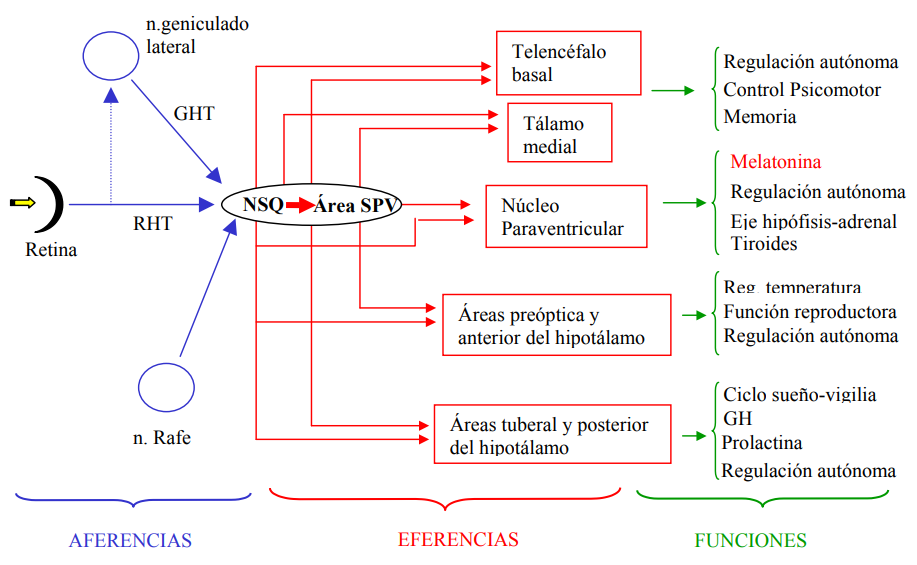
\includegraphics[scale=0.45]{Vias-NSQ.png}
\begin{footnotesize}	
	\caption{Esquema que representa las aferencias y eferencias principales del núcleo supraquiasmático
		(NSQ), así como algunas de las funciones que regula. Abreviaturas: RHT, tracto retino hipotalámico; GHT,
		trato genículo hipotalámico; NSQ, núcleo supraquiasmático; SVP, área supraparaventricular del tálamo.
		Modificado de Moore,1999.}
	\label{fig:EstructuraNSQ}
	\end{footnotesize}
\end{figure}



En la literatura científica se han propuesto dos principales mecanismos por los cuales los ritmos circadianos modifican la eficiencia de los procesos cognoscitivos  \cite{Valdez2014}; la primera sugiere que el reloj biológico genera oscilaciones en el sistema nervioso, lo que resulta en variaciones en el desempeño de todos los tipos de procesos. La segunda propone que el reloj biológico produce cambios en uno o más sistemas cerebrales específicos, que resultan en un cambio en los procesos cognoscitivos  específicos, lo que modula el desempeño en las tareas \cite{Valdez2014}.

Un ejemplo de esto es el estudio de \citeA{Faull2015}, donde evaluaron el flujo sanguíneo y la oxigenación cerebral de 30 participantes de 18 a 24 años en dos momentos del día (07:00 y 16:00 hrs) por medio de las técnicas de dopler transcraneal\footnote{El dopler transcraneal es una técnica que genera imágenes por ultrasonido de la cabeza por medio de ondas sonoras para producir fotografías del cerebro y del fluido cerebroespinal. Un ultrasonido Doppler transcraneal evalúa el flujo sanguíneo a través de las arterias más importantes del cerebro. El ultrasonido es seguro, no es invasivo, y no utiliza radiación ionizante.} y NIRS \footnote{La  espectroscopia del infrarrojo cercano cerebral (NIRS) es un método de imagenología no invasivo que consiste en la cuantificación de la atenuación de la luz del infrarrojo cercano (NIR). La luz del espectro NIR aprovecha la ventana óptica en la que la piel, los tejidos y los huesos son en su mayoría transparentes a la luz NIR en el espectro de 700-900 nm, mientras que la hemoglobina (Hb) y la hemoglobina desoxigenada (deoxi-Hb) son absorbentes de luz más fuertes. Las diferencias en los espectros de absorción de deoxi-Hb y oxi-Hb permiten la medición de los cambios relativos en la concentración de hemoglobina mediante el uso de la atenuación de la luz en múltiples longitudes de onda. Típicamente, el emisor y el detector de luz se colocan ipsilateralmente en el cráneo del sujeto.} 
Encontraron un mayor flujo sanguíneo cerebral por la tarde que por la mañana (214\rpm 37  [Mañana]  vs 261\rpm 103 $\mu$M x cm HHb\footnote{Abreviatura para Deoxihemoglobina} [tarde],  $ p< 0.01 $) y la oxigenación cerebral, mayor por la tarde comparado con la mañana (170\rpm 60 [Mañana]  vs 223\rpm 170 $\mu$ M x cm O\textsubscript{2}Hb\footnote{Abreviatura para Oxihemoglobina} [tarde], $p < 0.01$)

\subsection{Variaciones diurnas y cognición}
Se ha observado que los procesos cognoscitivos poseen una ciclicidad circadiana, es decir, existen variaciones en la eficiencia cognoscitiva a lo largo del día \cite{Valdez2012}. La evaluación de esta ciclicidad circadiana es por medio de las variaciones diurnas.

La diferencia entre ritmos circadianos y variaciones diurnas radica en que los ciclos circadianos tiene una duración aproximada de 24 horas, mientras que las variaciones diurnas delimitan al periodo de vigilia excluyendo las horas en que las personas duermen.

Para la evaluación de las variaciones diurnas de los procesos cognoscitivos (i.e. atención, memoria) se han empleado tres paradigmas, que se describirán a continuación.

\begin{enumerate}
	\item Protocolo de momento del día:
	Consiste en obtener respuestas a una misma tarea que son registradas múltiples veces y se buscan diferencias en la eficiencia a lo largo del día. Estas observaciones se realizan con personas en condiciones naturales, la mayoría durante el día y rara vez por la noche. Esto conlleva que los resultados de este tipo de estudios sean susceptibles a variables ambientales que podrían sincronizar o repercutir en los ritmos circadianos, como la luz, la temperatura ambiental,  la alimentación y la actividad física. Sin embargo, el empleo de este método ofrece ventajas cuando se desea estudiar las variaciones diurnas en ambientes naturales, y cuando las condiciones del laboratorio no permitan un control experimental estricto \cite{Blatter2007}.

	\item Protocolo de rutina constante:
	Para evitar la influencia de factores ambientales, los participantes pueden ser observados bajo condiciones constantes dentro del laboratorio controlando factores como temperatura ambiental, iluminación, consumo calórico y actividad física, por un periodo mayor a 24 horas, realizando tareas cognitivas o pruebas neuropsicológicas, cada una o dos horas durante el tiempo de observación \cite{Duffy2002}.

	\item De-sincronización forzada:
	Este método permite observar la participación de los ritmos circadianos al reducir o alargar los periodos de 24 horas del ciclo sueño-vigilia, de tal manera que se reajuste el reloj interno, obteniendo un desajuste entre el ciclo de sueño y la temperatura corporal (la cual continua oscilando en un periodo de 24 horas). En este protocolo los procesos cognoscitivos  son evaluados en diferentes momentos mientras las personas están despiertas, lo que permite identificar las variaciones circadianas de los procesos cognoscitivos  respecto al ciclo circadiano de la temperatura corporal \cite{Hanneman2001}.
\end{enumerate}

Los protocolos de rutina constante y de-sincronización forzada son los principales protocolos utilizados para evaluar ritmos circadianos para el estudio de las variaciones diurnas en los procesos cognoscitivos , dado que permiten un alto   control experimental pero están los participantes en un ambiente controlado muy diferente al estado natural, mientras que el protocolo de momento del día ofrece una aproximación al ambiente natural  de los individuos \cite{Valdez2014}.



Una aproximación más práctica, para el estudio de variaciones diurnas es la preferencia diurna o cronotipo,  evaluado por medio de cuestionarios de autorreporte como el cuestionario de matutinidad-vespertinidad de \citeA{Horne1976}, este cuestionario arroja una puntuación numérica en una escala entre extrema preferencia matutina y extrema preferencia vespertina. Por otro lado el Cuestionario de Cronotipo de Munich, el cual toma en cuenta las actividades en días laborales y no laborales para evaluar el cronotipo y la preferencia diurna, considerando los hábitos de sueño y la exposición a la luz de los sujetos, pero tiene la limitante de perder confiabilidad al calcular el cronotipo, si el sujeto usa despertador. Los puntajes de cronotipo evaluados por el  cuestionario de matutinidad-vespertinidad de \citeA{Horne1976} correlacionan significativamente con la fase circadiana de los individuos, por lo que se emplean como una variable que otorga una aproximación del funcionamiento del reloj biológico de los individuos \cite{Duffy,VonSchantz2015}.

\subsection{Efecto de las variaciones diurnas en la memoria de trabajo}

Uno de los primeros estudios de variaciones diurnas fue el estudio de  \citeA{Baddeley1970} en- que registraron a 38 sujetos en dos momentos del día, por la mañana (9:00 am-11:00 am)  y por la tarde(3:00 pm -5:00 pm). La tarea consistió en leer en voz alta a los participantes 24 secuencias de nueve dígitos aleatorios. Los sujetos tenían 11 segundos para repetir en el mismo orden la secuencia inmediatamente después de finalizado el ultimo dígito. La mitad de los participantes inició por la mañana las sesiones experimentales y la otra mitad por la tarde; esta asignación fue de manera aleatoria. Siete de las secuencias fueron idénticas, las restantes fueron diferentes entre sí. Los sujetos fueron más eficientes en recordar los elementos idénticos.
Adicionalmente, se encuentra que los participantes en el turno de la mañana cometen menos errores al recordar las secuencias en comparación con el turno de la tarde.
De este modo se observa que existen diferencias en la eficiencia de la memoria en función del momento del día.


Por otro lado, más recientemente la ciclicidad circadiana de la memoria de trabajo fue mostrada por \citeA{Ramirez2006} a través de un estudio en que evaluó a ocho estudiantes mujeres de 16 a 19 años con dos tareas, una fonológica y una visoespacial.
Se les aplicó un instrumento para evaluar su nivel subjetivo de cansancio y somnolencia.
En la tarea fonológica se presentaban cuatro letras en las esquinas de la pantalla como estímulo muestra y después durante el estímulo prueba se presentó una letra al centro,  %y un punto de fijación al centro, posterior a ello desaparecían las letras periféricas, el punto de fijación cambiaba a un número a manera de interferencia y cambiando nuevamente a una letra, 
debiendo responder si dicha letra se presentó en el arreglo anterior o no.
Por otro lado, en la tarea visoespacial se presentaban tres círculos negros ubicados en distintas posiciones de la pantalla %de tres a seis grados del punto de fijación; posterior a ello, desaparecían y, al igual a la tarea anterior, se presentaba un número a manera de interferencia, después éste desaparecía
 en estímulo de prueba se presentaron círculos blancos distribuidos por la pantalla. En esta tarea los participantes debían indicar si alguno de los círculos blancos coincidía con la ubicación de cualquiera de los círculos negros. El estudio tuvo una duración de 30 hrs y las mediciones se realizaron cada hora.
La proporción de respuestas correctas para las tareas fonológica y visoespacial variaron a lo largo del día. El valor mínimo de respuestas correctas para la tarea fonológica ocurrió a las 04:24 \rpm 1.03 hrs, teniendo el 9.91 \rpm 2.71\% de respuestas correctas. Mientras que para  la tarea visoespacial se obtuvo un mínimo de respuestas correctas a las 06:13 \rpm 0:25, con el 4.82 \rpm 2.54\%. Sin embargo, aunque la somnolencia fluctuó a lo largo del día, el cansancio aumentó en el trascurso del experimento, ya que las participantes permanecieron despiertas durante las 30 horas, lo que puede estar explicando el decremento en la eficiencia de los componentes (visoespacial y fonológico) de la memoria de trabajo. Cabe señalar que el detrimento de la memoria de trabajo se presentó en las primeras horas del día, después de la privación de sueño.


\citeA{Schmidt2015} reportaron que la eficiencia cognitiva puede variar a lo largo del día dependiendo del cronotipo, así como la activación de distintas áreas cerebrales, principalmente la corteza prefrontal. Por medio de un estudio en el que se evaluaron a 32 sujetos sanos en dos momentos del día, por la mañana y la noche, utilizando una tarea N-back  con tres niveles de dificultad (0-Back, 2-Back, 3-Back) durante un escaneo de fMRI. Únicamente, se observaron diferencias en la condición de mayor dificultad (3-Back) en comparación con los niveles de menor dificultad.
Los participantes con cronotipo vespertino tuvieron mayor porcentaje de respuestas correctas en la condición de 3-Back durante la tarde, comparado con los participantes con cronotipo matutino.
En cuanto a los resultados de fMRI, de igual manera sólo se observaron diferencias  entre participantes de cronotipos distintos en la condición de 3-Back. Se observó una mayor activación en el tálamo de los participantes con cronotipo vespertino durante la realización de la tarea por la tarde comparado con la mañana. Y en el giro frontal medial de los participantes con cronotipo matutino durante la mañana comparado con la realización de la tarea por la tarde. Lo cual muestra que el cronotipo influye en la  facilidad para realizar tareas cognitivas en el momento del día, es decir, hay mayor eficiencia para los matutinos por la mañana, y los vespertinos por la tarde. Así como también hay una activación diferencial a lo largo del día dependiente del cronotipo, por lo que no es claro si los efectos encontrados se deben al cronotipo o a la hora del día.


%\citeA{DelAngel2015} realizaron un experimento modificando los ciclos-sueño vigilia de los participantes con tres diferentes condiciones. En la primera de ellas se les indicó dormir el tiempo usual que dormían en condiciones normales (condición control), durante seis días. En la siguiente condición, con una duración de cinco días, se les pidió a los participantes reducir el tiempo de sueño a cuatro horas al día, de 02:00 am a 06:00 am. En la última condición se les indicó dormir libremente la noche posterior a la manipulación del ciclo sueño-vigilia, a manera de recuperación. La evaluación del desempeño se realizó por medio de tareas N-back, una auditiva y una visual, con tres niveles de dificultad; 0-Back, 1-Back, 2-Back. Las tareas se aplicaron a las 13:00 hrs para cada condición, un día antes de la reducción de sueño; tres días durante el periodo de reducción de sueño (primer, cuarto y quinto día) y un día después de la noche de sueño libre. \\
%%Los estímulos de la tarea auditiva consistieron en silabas, debiendo indicar si la silaba se presentó N  silabas antes. Los estímulos de la tarea visual consistieron en cuadros negros en alguna las esquinas de la pantalla, debiendo indicar los participantes si el cuadro negro se ubicaba en la misma esquina que N ensayos atrás.

%Para las tareas auditivas se encontraron un decremento en el porcentaje de respuestas correctas en 0-back y 2-back en el quinto día de privación de sueño, y sólo para 2-back el día de posterior a la noche de sueño libre; con respecto a la condición control.
%No se encontraron diferencias en los tiempos de reacción. \\
%Para las tareas visuales se encontraron únicamente diferencias en la condición de 2-Back, se observaron diferencias en el porcentaje de respuestas correctas en el primer y quinto día de reducción de sueño comparado con la condición control. Adicionalmente, se encontraron diferencias en los tiempos de reacción en el primer, cuarto y quinto día de reducción de sueño con respecto a la condición control.

%Este estudio muestra que la alteración en el ciclo sueño-vigilia (privación de sueño) modifica la eficiencia del componente fonológico de la memoria de trabajo y que es suficiente una noche de recuperación para regresar al estado normal, como sugiere el decremento al día posterior a la noche libre. Este decremento puede afectar la capacidad de procesar información lingüística, repercutiendo en el desempeño de tareas verbales, así como entender y procesar texto escrito.
%Además, se observa que hay una disminución en la eficiencia del componente visoespacial de la memoria de trabajo, lo cual podría repercutir en un mayor esfuerzo para procesar imágenes, localizar objetos en el espacio y resolver problemas que requieren procesamiento visual. Pero los efectos observados podrían deberse más a el efecto del sueño que a variaciones diurnas.

Sin embargo, estos estudios no hacen una comparación de los componentes de la memoria de trabajo (i.e. mantenimiento y manipulación), por lo que se desconoce si ambos o sólo alguno de ellos se ve afectado por las variaciones diurnas.

\section{Justificación}
La memoria de trabajo es, como se ha descrito, un intermediario entre el entorno externo y los procesos de aprendizaje y memoria a largo plazo. Por lo que el conocer el mecanismo en que la ejecución y eficiencia de la memoria de trabajo se ve afectada por el momento del día en que se realiza una tarea cognoscitiva, de manera independiente a una modificación del ciclo sueño-vigilia, aportaría más información respecto a la variación diurna de ésta en condiciones naturales. 

Con esta investigación se pretendió conocer el efecto del momento del día sobre la eficiencia para mantener y manipular información en la memoria de trabajo.

\section{Planteamiento del problema}
Se sabe que la memoria de trabajo es un almacén de información temporal, conformado por dos componentes, el  mantenimiento y la manipulación de información. Existen variaciones en la eficiencia a lo largo del día que son dependientes del cronotipo. Sin embargo, no sabemos si estas variaciones se dan en ambos componentes de la memoria de trabajo o sólo en alguno de ellos. También predominan los estudios que evalúan las variaciones diurnas de la memoria de trabajo en donde se realiza una modificación del ciclo sueño-vigilia, al igual que estudios que evalúan las variaciones en función del cronotipo por lo que los resultados observados podrían deberse a esa manipulación del sueño vigilia o del cronotipo, más que a la variación natural. %Para ello en la presente tesis, se busco evaluar la memoria de trabajo y sus componentes utilizando el paradigma de momentos del día.

\section{Pregunta de Investigación}
¿Existen diferencias en la eficiencia para mantener y manipular información en la memoria de trabajo en función del momento del día?

\section{Hipótesis}
Las personas evaluadas en distintos momentos del día, independientemente de su cronotipo, muestran mayor capacidad para el mantenimiento y manipulación de la información por la mañana que disminuye a lo largo del día hasta el anochecer, siendo más eficientes para mantener que para manipular.
%Cuando las personas son evaluadas en distintos momentos del día, muestran mayor capacidad para el mantenimiento y manipulación de la información por la mañana que disminuye a lo largo del día hasta alcanzar la noche. Siendo más eficientes para mantener que para manipular.

\section{Objetivo general}
Evaluar si se diferencia la eficiencia de la memoria de trabajo es diferente en distintos momentos del día.
\subsection{Objetivo específico}
Evaluar la capacidad para mantener y manipular información en la memoria de trabajo  por la mañana, por la tarde y por la noche en jóvenes sanos de 20 a 30 años de edad. %personas sanas de 20 a 30 años, sin antecedentes neurológicos ni psiquiátricos, sin historial de consumo de drogas ilícitas ni dependencia a drogas lícitas en los últimos 12 meses.

\newpage

\section{Método}
\subsection{Participantes}
En el estudio participaron 59 jóvenes (29 hombres y 30 mujeres) que fueron reclutados mediante un muestreo no probabilístico. Los criterios de inclusión fueron tener entre 20 y 30 años, escolaridad mínima de 12 años, ser diestro, tener visión normal o corregida, no haber consumido alguna droga ilícita al menos en los últimos 12 meses, no presentar ni haber presentado dependencia a ninguna droga, no padecer o tener antecedentes directos de enfermedades neurológicas y/o psiquiátricas, no presentar niveles severos de depresión y/o ansiedad. Cuando se detectó que el participante cubría los criterios de inclusión, se le asignó a uno de tres grupos (7 hrs, 12 hrs y 19 hrs.) de manera semialeatoria con el fin de balancear el cronotipo y sexo entre grupos.

\subsection{Materiales y aparatos}
Se utilizó una computadora con el software E-Prime V.1.2 \textit{\cite{PsychologySoftwareTools2012}} para la presentación de las tareas,  el registro de la conducta, y el tiempo de reacción en milisegundos (ms). Los participantes respondieron a las tareas por medio de dos cajas de respuesta (una izquierda y una derecha).

\subsubsection{Instrumentos}
\paragraph{Carta de consentimiento informado} \mbox{}\\
Es un documento en donde se explica a los participantes la justificación del estudio, los objetivos, los beneficios y el procedimiento que se llevará a cabo en la sesión experimental. Se explica  que la decisión de participar es completamente voluntaria y que puede retirarse, sin alguna consecuencia negativa, si en algún momento así lo desea. Se explica que todos los datos obtenidos serán confidenciales y que únicamente serán utilizados para fines de la investigación. %(Está carta esta siendo evaluada por el comité de ética de la Facultad de Psicología, UNAM)

\paragraph{Cuestionario de datos generales} \mbox{}\\
Este cuestionario permite adquirir datos generales de los participantes (e. g., nombre completo, edad, teléfono, domicilio, nivel de escolaridad, presencia de alguna enfermedad neurológica o psiquiatra en él o en familiares de línea directa, etc.).

\paragraph[Inventario de Edimburgo]{Inventario de Edimburgo \cite{Oldfield1971}} \mbox{}\\
Este inventario permite evaluar si el sujeto es diestro, ambidiestro o zurdo. Son 12 preguntas acerca del uso preferente de su mano u otras partes del cuerpo a ciertas actividades. Los puntajes obtenidos pueden ser de -100 a +100. El puntaje de -100 a -40 indica una lateralidad zurda. De -41 a 39 indica una ambidiestra y de 40 a 100 indica una lateralidad diestra. Participaron sólo participantes con lateralidad diestra

\paragraph{Cuestionario de uso de sustancias} \mbox{}\\
Este cuestionario permite detectar si el participante ha consumido o consumió alguna droga (e. g., tabaco, alcohol, marihuana, narcóticos, alucinógenos, tranquilizantes, esteroides, sustancias naturistas, bebidas energizantes o alguna otra sustancia). Se realizará un cuestionario aparte para detectar la presencia de trastorno de abuso de sustancias, si el participante ha consumido alguna droga más de 12 veces en un periodo de 12 meses. Participaron aquellos que no presentaron consumo de sustancias ilícitas ni trastorno por uso de sustancias en el ultimo año. %de aquí lo difícil de completar la muestra

\paragraph[Inventario de depresión de Beck]{Inventario de depresión de Beck \cite{Jurado1998}} \mbox{}\\
Es un inventario autoaplicable de lápiz y papel, estandarizado para población mexicana, que proporciona una medida de la presencia y de la gravedad de sintomatología asociada a depresión en adultos y adolescentes de 13 años en adelante. Se compone de 21 ítems, cada ítem se responde en una escala de 4 puntos, de 0 a 3. Estos ítems indican síntomas asociados a la depresión como tristeza, llanto, pérdida del placer, sentimientos de fracaso y culpa, pensamientos o deseos suicidas y pesimismo. El puntaje máximo que se puede obtener es de 63 puntos. Este instrumento establece niveles de depresión dependiendo del puntaje: 0-9, ausencia de depresión; 10-16, depresión leve; 17-29, depresión moderada y de 30 a 63, depresión grave. Los participantes deben elegir el reactivo que describa mejor cómo se ha sentido en la última semana, incluyendo el día de la aplicación. Los participantes que obtuvieron un puntaje mayor o igual a 30 fueron excluidos de la investigación.

\paragraph[Inventario de ansiedad de Beck]{Inventario de ansiedad de Beck \cite{Robles2001}} \mbox{}\\
Es un inventario autoaplicable de lápiz papel,  estandarizado para población mexicana, que proporciona una medida de presencia y gravedad de síntomas asociados a la ansiedad en adultos y adolescentes de 13 años en adelante. Se compone de 21 ítems, cada ítem se puntúa de 0 a 3, correspondiendo la puntuación 0 a “nada o poco”; 1 a “más o menos”; 2 “moderadamente” y 3 “severamente”.  El puntaje máximo que se puede obtener es de 63 puntos. Este instrumento establece niveles de ansiedad dependiendo del puntaje: 0-4, ansiedad mínima; 5-15, ansiedad leve; 16-30, ansiedad moderada; 31-63, ansiedad severa. Los participantes deberán elegir  la opción que describa mejor cómo se ha sentido en la última semana, incluyendo el día de la aplicación. Los participantes que obtuvieron un puntaje mayor o igual a 30 fueron excluidos de la investigación.

\paragraph[Subescala de retención de WAIS-III ]{Subescala de retención de WAIS-III \cite{WeschlerIII2004}} \mbox{}\\
Esta subescala permitió evaluar si la capacidad de la memoria de trabajo se encuentra en rangos normales de acuerdo a la edad cronológica. Se utilizó como medida control para realizar una comparación con los resultados obtenidos en las tareas experimentales. Esta escala consta de dos partes presentadas de manera verbal a los participantes, la primera parte consiste en grupos de tres a nueve dígitos y se le indica repetirlos en el mismo orden. En la segunda parte se presenta al participante grupos de dos a ocho dígitos que ha de repetir en orden inverso al que escucharon estos dígitos.
Está prueba se uso como control adicional a las tareas de memoria de trabajo.


\paragraph[Escala breve de inteligencia Shipley-2]{Escala breve de inteligencia Shipley-2 \cite{Shipley2014}} \mbox{}\\
Esta prueba permite evaluar de manera breve y eficaz la inteligencia en niños, adolescentes y adultos, mediante la evaluación de dos tipos de inteligencia (fluida y cristalizada), que proporcionan una estimación rápida de la Inteligencia general.
Se compone de tres subpruebas: Vocabulario, que mide habilidades cristalizadas; y Abstracción y Bloques, que mide las habilidades fluidas. Por medio de las subpruebas se amplía el alcance de la evaluación y se obtienen puntuaciones combinadas. El instrumento, debido a su brevedad, permite una aplicación rápida (22 minutos máximo). Únicamente se emplearon las subpruebas de vocabulario y de abstracción, ya que sólo requieren para su realización la utilización de lápiz y papel. No se empleó la prueba de bloques, ya que está diseñada para utilizarse en población analfabeta.
Este cuestionario se utilizo como un dato de referencia para la inteligencia de nuestros participantes

\paragraph[Cuestionario de matutinidad-vespertinidad% de Horne y Östberg
]{Cuestionario de matutinidad-vespertinidad \cite{Horne1976}.} \mbox{}\\
Este cuestionario de autorreporte consta de cinco reactivos para obtener un puntaje máximo de 25. El instrumento evalúa el cronotipo dependiendo del puntaje: de 4-7, extrema preferencia vespertina; 8-11, preferencia vespertina; 12-17, preferencia indiferenciada; 18-21, preferencia matutina; 2-25, extrema preferencia matutina.
Este cuestionario se utilizó como un instrumento exploratorio a fin de conocer el cronotipo de los participantes.


\subsection{Estímulos}
Se utilizaron 40 estímulos conformados por figuras irregulares que no representan un estímulo conocido, con la finalidad de medir la capacidad para el mantenimiento y manipulación. %Esto permite evaluar la capacidad de mantener y manipular información, sin que la medición se vea afectada o sesgada por un conocimiento previo de las formas
Estos estímulos se presentaron en dos tonalidades de gris (RGB \textless sigla en inglés de red, green, blue\textgreater{}: 100,100,100 y RGB: 150,150,150) ubicados sobre un fondo gris claro (RGB: 200,200,200), a fin de  evitar que se generen postimagen.\footnote{Es una imagen ``residual'' por el estímulo directo de un color, pero no se encuentra presente. Ocurre cuando se observa durante un tiempo una superficie de color y luego se desliza el ojo rápidamente sobre una superficie gris o blanca. En este caso se vería en segundo lugar el color complementario u opuesto al observado en primer lugar; de rojo por ejemplo, la imagen posterior será verde azulado. La postimagen, tiene una explicación física. Los conos de nuestros ojos son los receptores encargados de percibir el color, estos receptores contienen neuronas que pueden ``fatigarse'' ante un estímulo continuo. Lo que sucede es que cuando estás neuronas se fatigan ante un determinado color, producen su negativo.}

\subsection{Tareas experimentales}

Se aplicaron tres tareas con la finalidad de evaluar la capacidad de mantenimiento y manipulación de la memoria de trabajo, las cuales se presentaron a los participantes en un monitor de computadora a un metro de distancia.: Una tarea control, una de mantenimiento y otra de manipulación. Las tareas estuvieron contrabalanceadas entre sujetos para evitar el efecto de aprendizaje y familiaridad con las tareas.

\subsubsection{Tarea control}
Esta tarea constó de 80 ensayos divididos en dos bloques de 40 ensayos por bloque. El orden de presentación de los estímulos fue de manera aleatoria y contrabalanceada. Cada ensayo estaba conformado de la siguiente manera, un punto de fijación, una primer figura como estímulo clave, una cruz como punto de fijación, y una segunda figura como estímulo prueba, seguido de un otro punto de fijación y un tono que indica el inicio de un nuevo ensayo.
(Ver Figura~\ref{fig:EstruturaEnsayo}).


En el primer bloque, los participantes debían presionar el botón izquierdo al aparecer la segunda figura; y el botón derecho al aparecer la segunda figura en el segundo bloque. Esto estaba contrabalanceado entre sujetos. Esta es una tarea control porque los participantes no deben realizar ningún mantenimiento o manipulación de los estímulos presentados, debiendo únicamente presionar un botón determinado al aparecer la segunda figura.

\begin{figure}[ht]
	\centering
	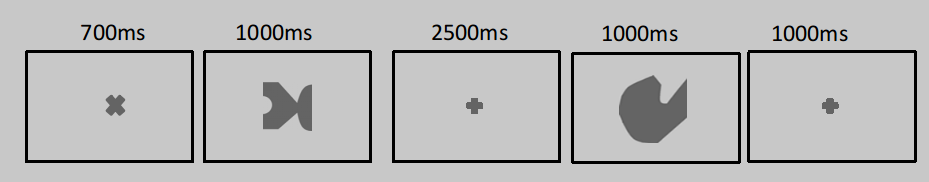
\includegraphics[scale=0.5]{ensayoMT.png}
	\caption{Estructura y pantallas presentadas durante los ensayos. Se presenta un tache como primer punto de fijación por 700ms, una primer figura por 1000ms, seguido de una cruz como punto de fijación por 2500ms, una segunda figura por 1000ms  (donde el participante da su respuesta) y finalmente una cruz como punto de fijación por 1000ms.}
	\label{fig:EstruturaEnsayo}
\end{figure}


\subsubsection{Tarea de mantenimiento}
Para evaluar la capacidad de mantenimiento se diseñó una tarea, la cual consta de 80 ensayos divididos en cuatro bloques de 20 ensayos por bloque.  Semejante a la tarea control en la estructura del ensayo. El participante   debe indicar si el estímulo prueba con respecto al estímulo clave conserva el mismo color y forma. El orden de presentación de los estímulos es de manera aleatoria y contrabalanceada.
%Los participantes deberán determinar si cuando aparece un círculo la segunda figura conserva el color (Baja Dificultad) y si aparece un tache debe determinar si la segunda figura conserva el color y forma, con respecto a la primera figura. (Alta Dificultad).\\
%De la misma manera, la otra mitad de los participantes deberá determinar si cuando aparece un tache la segunda figura conserva el color y si aparece un círculo debe determinar si la segunda figura conserva el color y forma, con respecto a la primera figura.
Los participantes debían responder presionando un botón según si se conserva o no, el color y la forma (Figura~\ref{fig:str-mt}).
De estos 80 ensayos, 40 fueron target (cumple el criterio de color y forma) y 40 non-target (no cumple el criterio color y forma). %De estos 80, 40 son de alta dificultad y 40 de baja dificultad.

\begin{figure}[h]
	\centering
	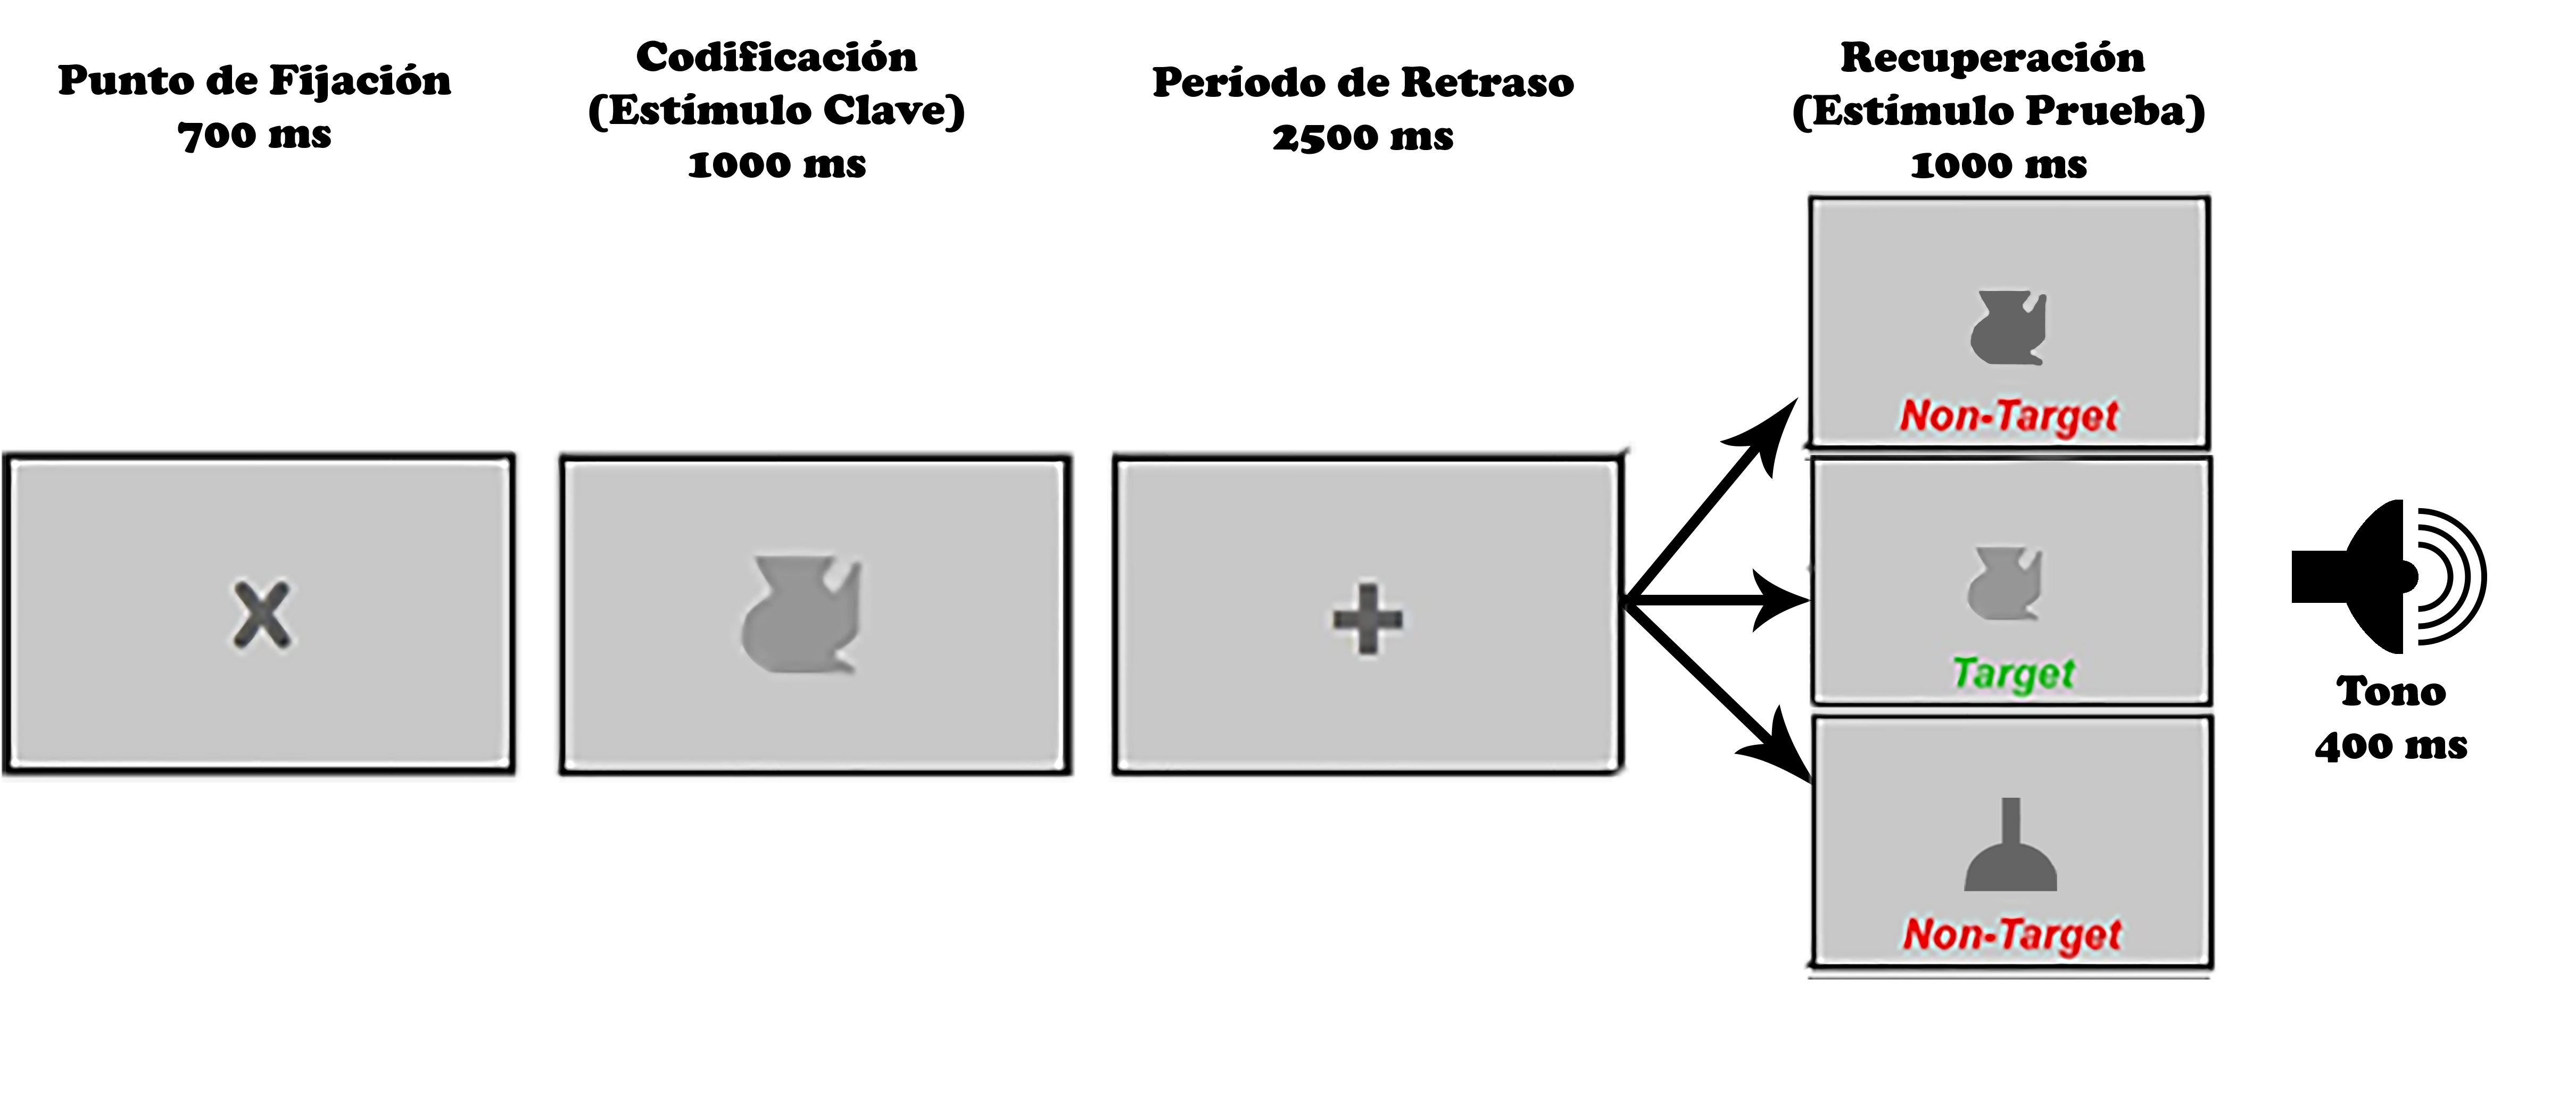
\includegraphics[scale=0.35]{str-mt.png}
	\caption{Esquema de la tarea de mantenimiento: orden y tipos de ensayo.}
	\label{fig:str-mt}
\end{figure}

\subsubsection{Tarea de manipulación}
Para evaluar la capacidad de manipulación, se diseñó una tarea con la misma estructura que las tareas anteriores con la diferencia que el participante debía determinar si la rotación del estímulo prueba era o no de \ang{180}, en dirección a las manecillas del reloj, con respecto al estímulo clave. El orden de presentación de los estímulos fue de manera aleatoria y contrabalanceada (Figura~\ref{fig:str-mp}). 

Los participantes debían responder presionando un botón según si se cumple el criterio de rotación o no.
De igual forma que en las tarea anteriores, de los 80 ensayos, 40 son target (cumple el criterio de rotación de \ang{180}) y 40 non-target (no cumple el criterio de rotación de  \ang{180}). %De estos 80, 40 son de alta dificultad y 40 de baja dificultad.

\begin{figure}[h!]
	\centering
	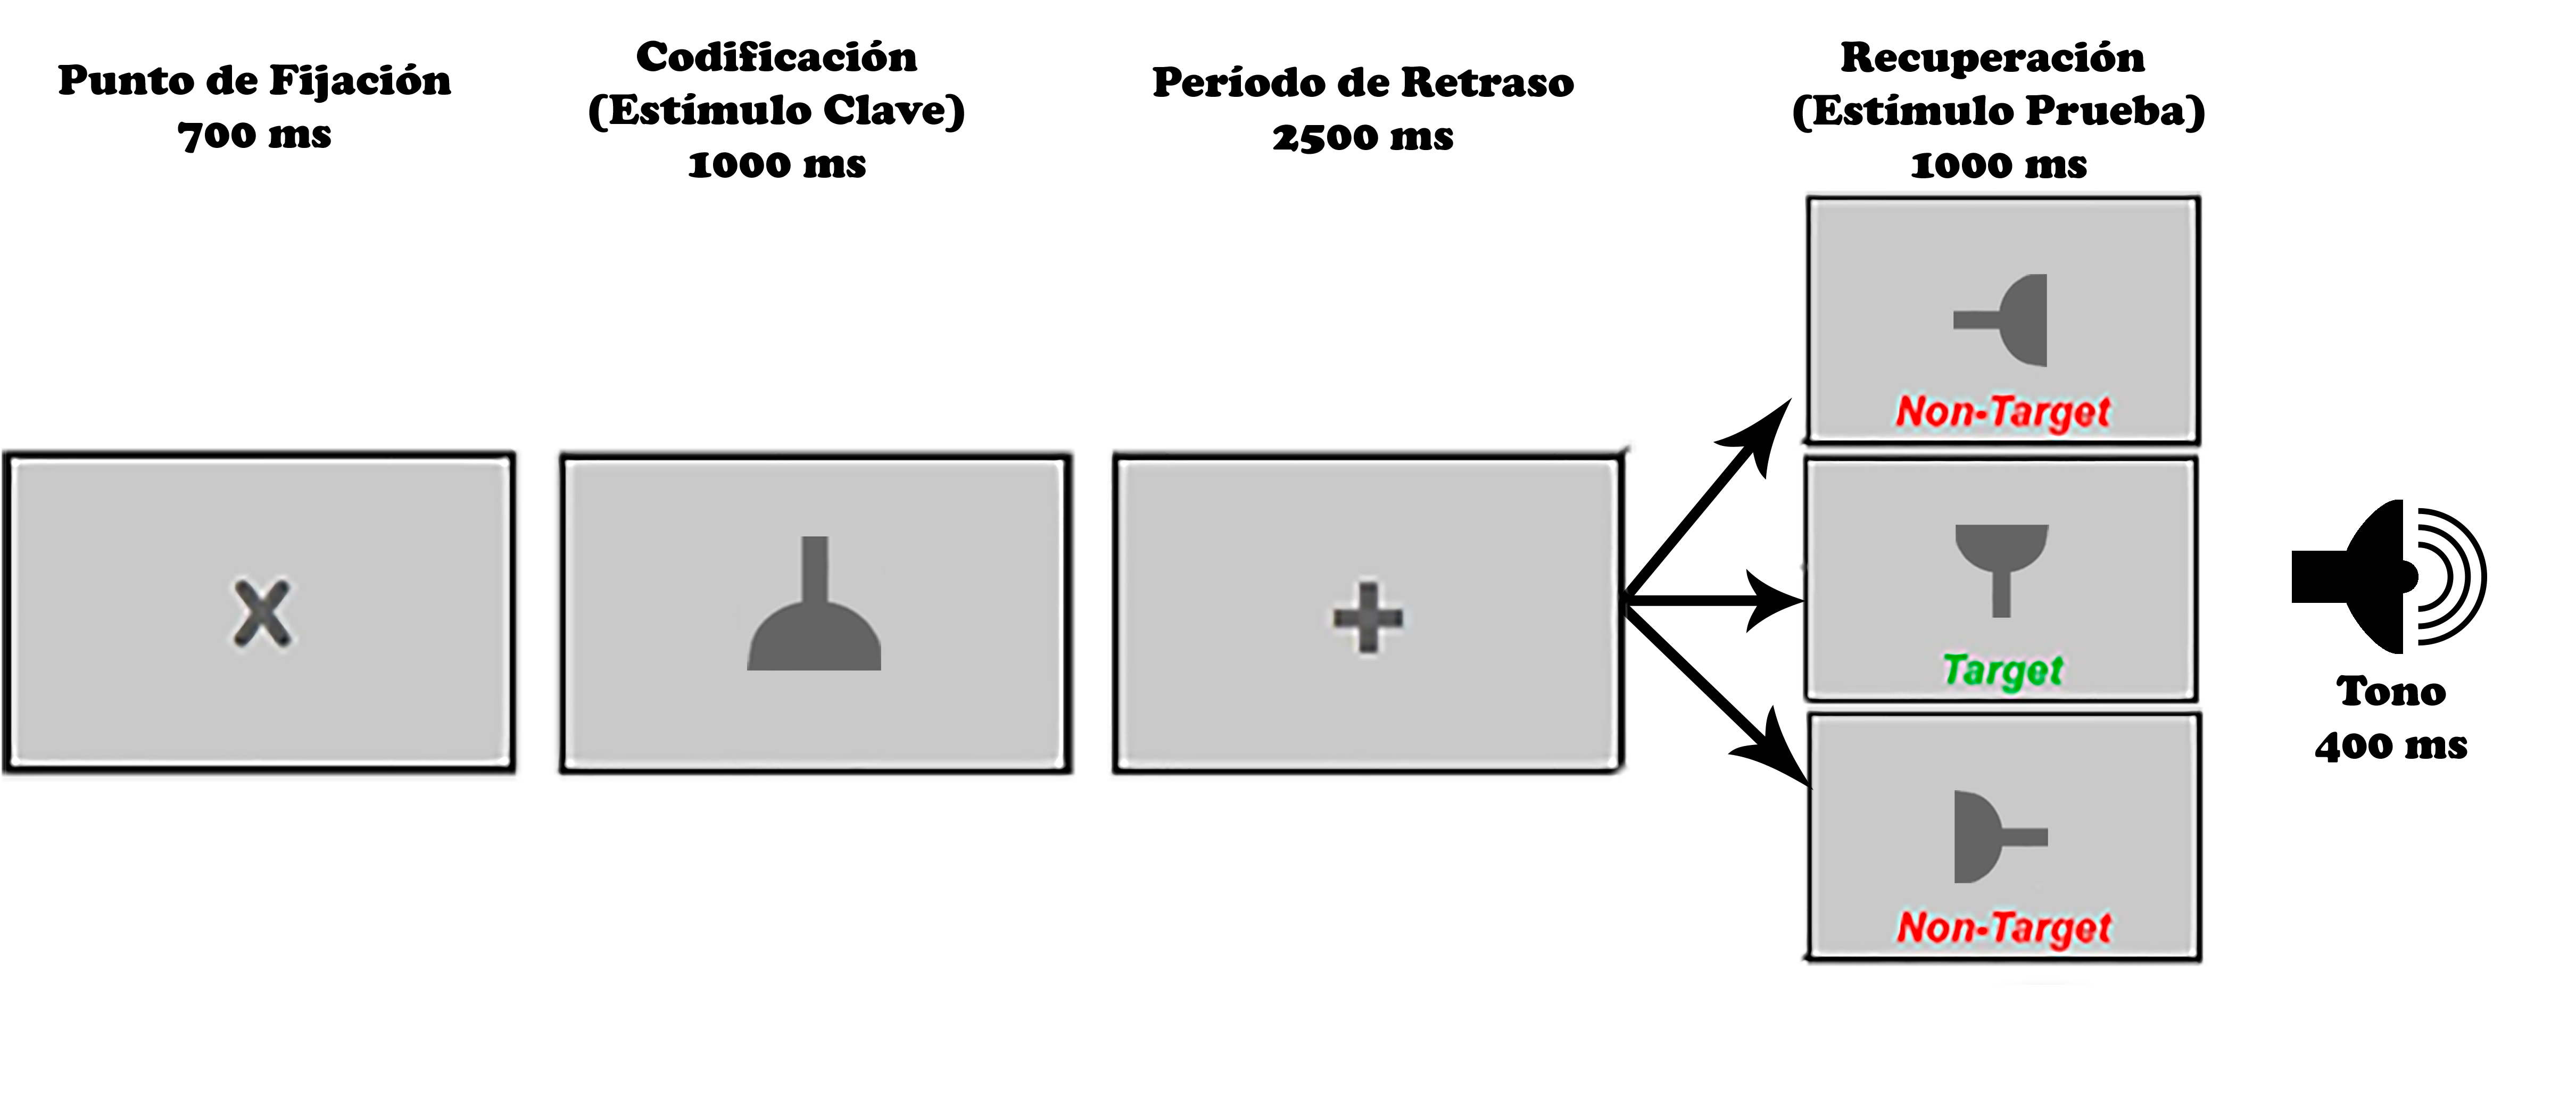
\includegraphics[scale=0.09]{str-mp.png}
	\caption{Esquema de la tarea de manipulación: orden y tipos de ensayo.}
	\label{fig:str-mp}
\end{figure}

{\setstretch{1.35}
\subsection{Procedimiento}
Las sesiones experimentales se realizaron en tres momentos del día, por la mañana de 7:00 am a 9:00 am, por la tarde de 12:00 pm a 02:00 pm y por la noche de 7:00 pm a 9:00 pm. Para cada momento del día, 10 hombres y 10 mujeres realizaron  las tres tareas, con excepción del turno matutino donde participaron 10 mujeres y 9 hombres, teniendo una muestra total de 59 participantes.

La sesión comenzó con la entrevista inicial donde se aplicaron los instrumentos antes descritos, con la finalidad de verificar el cumplimiento de los criterios de inclusión, posteriormente los participantes realizaron las tareas. Las tareas de mantenimiento y manipulación se contrabalancearon entre sujetos; la tarea control siempre fue la primera en realizarse para todos los participantes para evitar un efecto de memoria en la condición control.
}
{\setstretch{1.35}
\subsection{Análisis Estadístico}
Se analizaron las respuestas correctas, indice d'\footnote{El indice de discriminación d’(\textit{"de Prima"}) 
permite tener una medida de eficiencia más certera, ya que el porcentaje de respuestas correctas no siempre refleja eficiencia, un participante podría siempre presionar el botón que indica que el estímulo prueba mantuvo el color y la forma o fue rotado \ang{180}, dependiendo de la condición, sin importar si el estímulo realmente fue igual o cumplió con las condiciones, y se obtendría así un 100\% de respuestas correctas \cite{Haatveit2010}. De ahí la importancia de considerar las respuestas correctas y las falsas alarmas al estímulo non-target. La obtención de d’ se calcula de la resta del puntaje Z de los aciertos menos el puntaje Z de las falsas alarmas.}
%permite tener una medida de eficiencia más certera, ya que permite la discriminación de los ensayos targets y los non-target  y no solo toma en cuenta las respuestas correctas, sino, la capacidad de discriminar de nuestros participantes.  La obtención de d’ se calcula de la resta del puntaje Z de los aciertos menos el puntaje Z de las falsas alarmas.} 
y tiempos de reacción de las mismas. Se realizó el análisis de resultados  por medio de un análisis de varianza (ANOVA) mixto (3x2) tomando en consideración los tres momentos del día (mañana, tarde y noche) como factor entre grupos; y, las tareas de mantenimiento y manipulación como factor intragrupo.
Los resultados se consideraron significativos a partir de $ p\textless0.05$, en caso de obtener resultados significativos, se empleó la prueba Tukey para muestras desiguales como post hoc.
}
\newpage

\section{Resultados}
\subsection{Descripción de la muestra}
Cincuenta y nueve sujetos participaron en esta investigación y fueron  agrupados en tres diferentes horarios (turno). En la tabla \ref{tab:CaracSoci} se muestran las características socio-demográficas de cada uno de estos grupos. La variable Horas de Sueño fue significativamente diferente entre grupos por lo que se realizó un análisis de covarianza en los análisis de eficiencia en las tareas de memoria de trabajo incluyendo la hora de sueño como covariable. 

\begin{table}[h!]
 \begin{threeparttable}
\caption{Características Socio-demográficas de la Muestra}
\footnotesize
\begin{tabular}{|p{0.24\linewidth}|c|c|c|c|c|}
\hline  & \multicolumn{3}{c|}{Grupo (Turno)} & Prueba Estadística & $p$ \\ 
\hline  & Mañana & Tarde & Noche &  &  \\ 
\hline N & 19 & 20 & 20 &  &  \\ 
\hline Hombres/Mujeres & 9/10 & 10/10 & 10/10 & $\chi^{2}= 0.35 $ & $0.95$ \\ 
\hline Edad (años; Media \rpm DE) & 21.73 \rpm 0.40 & 21.95 \rpm 0.39 & 22.6 \rpm 0.39 & $F (2, 56)= 1.28$	 & $0.28$ \\ 
\hline Escolaridad 
(años; Media \rpm DE) & 15.57 \rpm 0.28 & 15.26 \rpm 0.27 & 15.90 \rpm 0.27 & $F (2, 56)= 1.34$ & $0.26$ \\ 
\hline Edimburgo [Mediana (rango)]	 & 90 (75-100) & 83 (58-100) & 91 (40-100) & $H (2, 59)= 3.49$	 & $0.17$ \\ 
\hline Inventario de Depresión de Beck [Mediana (rango)] & 4 (0-14) & 6 (0-13) & 5 (0-15) & $H (2, 59)= 1.84$  & $0.39$ \\ 
\hline Inventario de Ansiedad 
de Beck [Mediana (rango)] & 4 (0-16) & 5 (0-9) & 4 (0-25) & $H (2,59)= 0.51$ & $0.77$ \\ 
\hline Retención de Dígitos  Subescala WAIS-IV  (Puntuación Natural; Media \rpm DE) & 14.6 \rpm 0.74 & 14.5 \rpm 0.74 & 14 \rpm 0.74 & $F (2, 56)= 0.18$	 & $0.83$ \\ 
\hline IMC (Media \rpm DE) & 24.63 \rpm 0.99 & 24.69 \rpm 0.96 & 23 \rpm 0.96 & $F (2, 56)= 1.0$ & $0.37$ \\ 
\hline Shipley (Media \rpm DE) & 113.21 \rpm 1.57 & 111.4 \rpm 1.53 &  110.85 \rpm 1.53 & $F (2, 56)= 0.62$ & $0.53$ \\ 
\hline Horas de sueño     (Media\rpm DE) & 5.37 \rpm 0.32 & 7.60 \rpm 0.32 & 6.93 \rpm 0.32 & $F (2, 56)= 12.21$ & $<0.01$ \\ 
\hline Horas de sueño habitual (Media\rpm DE) & 6.21 \rpm 0.26 & 6.22 \rpm 0.26 & 6.11 \rpm 0.26 & $F (2, 56)= 0.51$ & $0.95$ \\ 
\hline Temperatura    (Media\rpm DE) & 36.44 \rpm 0.07 & 36.62 \rpm 0.07 & 36.57 \rpm 0.07 & $F (2, 56)= 1.45$ & $0.24$ \\ 
\hline  Cronotipo  (Mat/Indet/Vesp) & 5/10/4  & 5/12/3 &  6/10/4 & $\chi^{2}= 2.37$ & $0.88$ \\ 
\hline Cronotipo Puntuación [Mediana(Rango)] & 14(9-21) & 16(8-21) & 14(8-22) & $H (2, 59)= 0.41$ & $0.81$ \\ 
\hline 

\end{tabular} 
 \begin{tablenotes}
      \footnotesize
      \item WAIS III: Subescala de retención de dígitos de la escala de inteligencia Weschler para adultos III;
      \item IMC: Índice de Masa corporal; DE: Desviación Estándar
      \label{tab:CaracSoci}
    \end{tablenotes}
    \end{threeparttable}

\end{table}

\subsection{Eficiencia en la Memoria de Trabajo}
En la tabla \ref{tab:resum} se muestra el resumen del \% de Respuestas correctas (RC), Indice d', y Tiempo de reacción (TR). A continuación se describen los hallazgos encontrados.

\begin{table}[h!]
\begin{center}
 \begin{threeparttable}
\caption{Media\rpm EEM del \% de RC, d', TR en función del grupo. \label{tab:resum} \index{tab}}
\begin{tabular}{|c|c|c|c|}
\hline 
Turno & \% Respuestas Correctas & d' & Tiempo de reacción  \\ 
\hline 
Mañana & 88.84\rpm 1.68 & 2.78\rpm 0.14 & 691.65\rpm 31.10  \\ 
\hline 
Tarde & 85.21 \rpm 1.64 & 2.51\rpm 0.14 & 748.18\rpm 30.31  \\ 
\hline 
Noche & 88.31\rpm 1.64 & 2.72\rpm 0.14 & 763.14\rpm 30.31 \\ 
\hline 
\end{tabular} 
 \begin{tablenotes}
      \footnotesize
      \item Media\rpm EEM
    \end{tablenotes}
    \end{threeparttable}

\end{center}
\end{table}

\subsubsection{Porcentaje de Respuestas Correctas}
Para el porcentaje de respuestas correctas se observaron diferencias significativas en función del subproceso, siendo mas eficientes para mantener que para manipular los sujetos (Mantenimiento vs. Manipulación; Fig. \ref{Sub:rctar}) $F (1,56)= 41.093, \eta_{p}^{2}= 0.42, *p\textless 0.01.$ No se observaron diferencias significativas en función del Turno (mañana, tarde y noche) ($p= 0.48$; Fig. \ref{Sub:rctur}), ni interacción Turno x Subproceso ($p=0.96.$ ;Fig. \ref{Sub:rcint}).


\begin{figure}[h]
 \begin{footnotesize}
  \begin{subfigure}[a]{.4\textwidth}	
	\centering
	\caption{Interacción de Factores}
	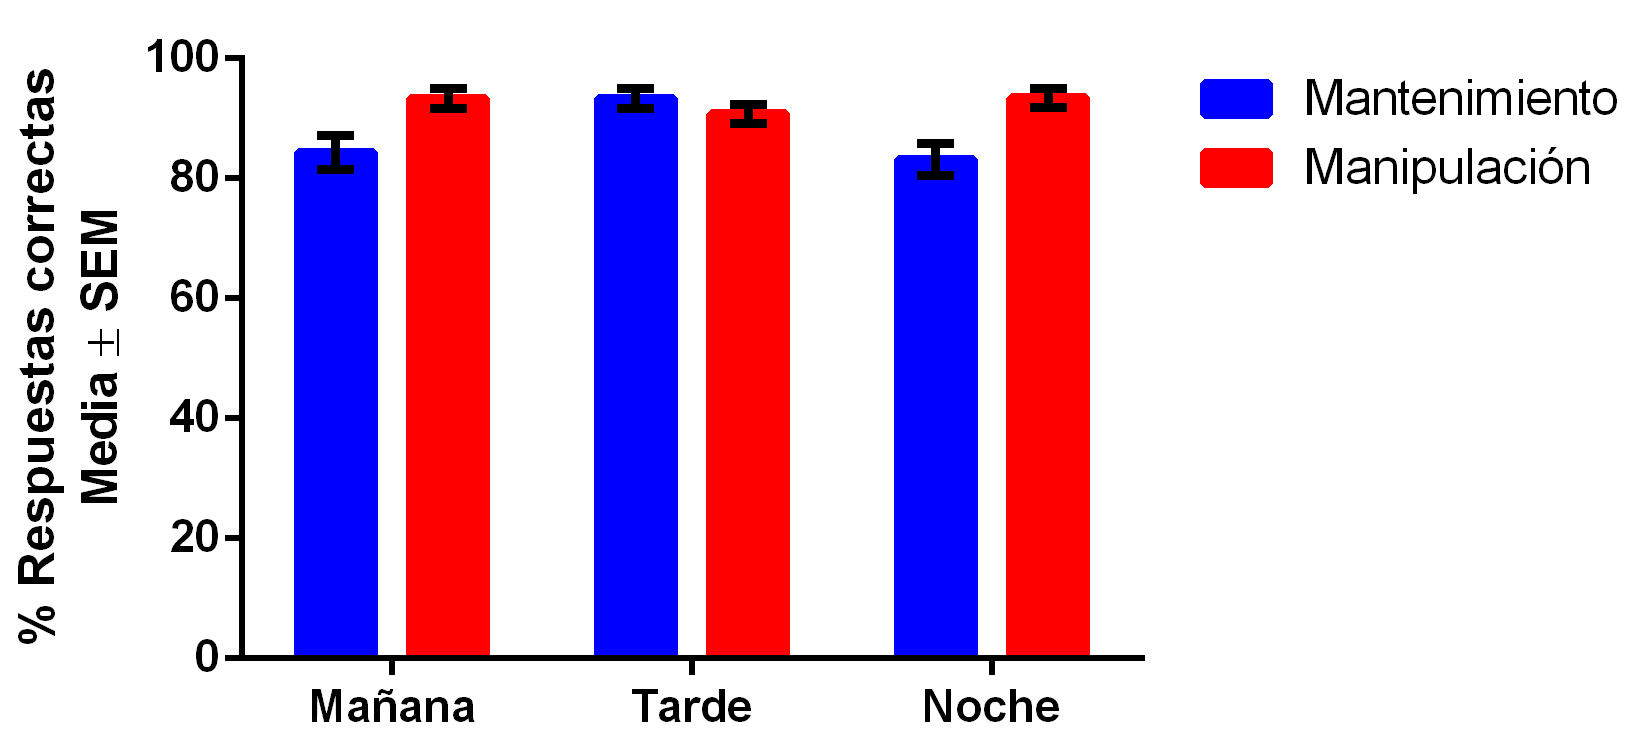
\includegraphics[scale=0.6]{graficas/RC_intr.png}	
	\label{Sub:rcint}
	\end{subfigure}
    \hfill
    \begin{subfigure}[a]{\textwidth}	
	\centering
	\caption{Entre turnos}
	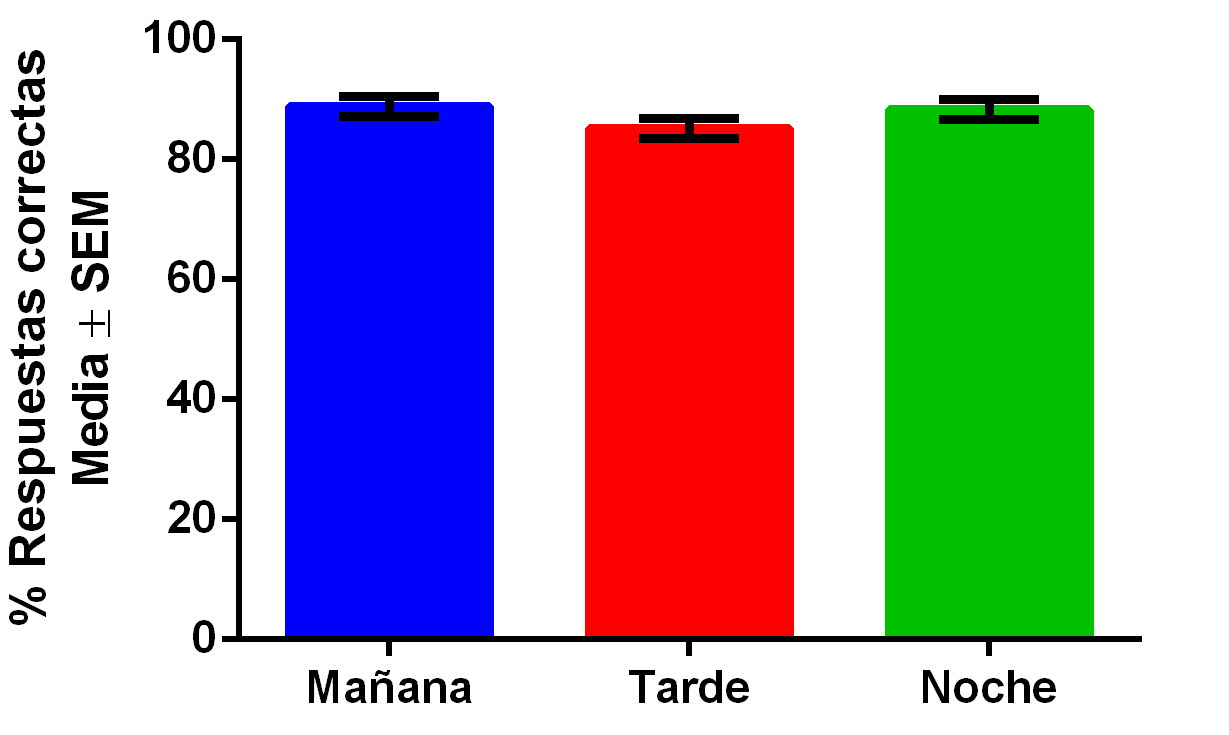
\includegraphics[scale=0.6]{graficas/RC_Tur.png}	
	\label{Sub:rctur}
	\end{subfigure}
	
	\begin{subfigure}[b]{0.9\textwidth}	
	\centering
	\caption{En función del subproceso (Mantenimiento vs. Manipulación).}
	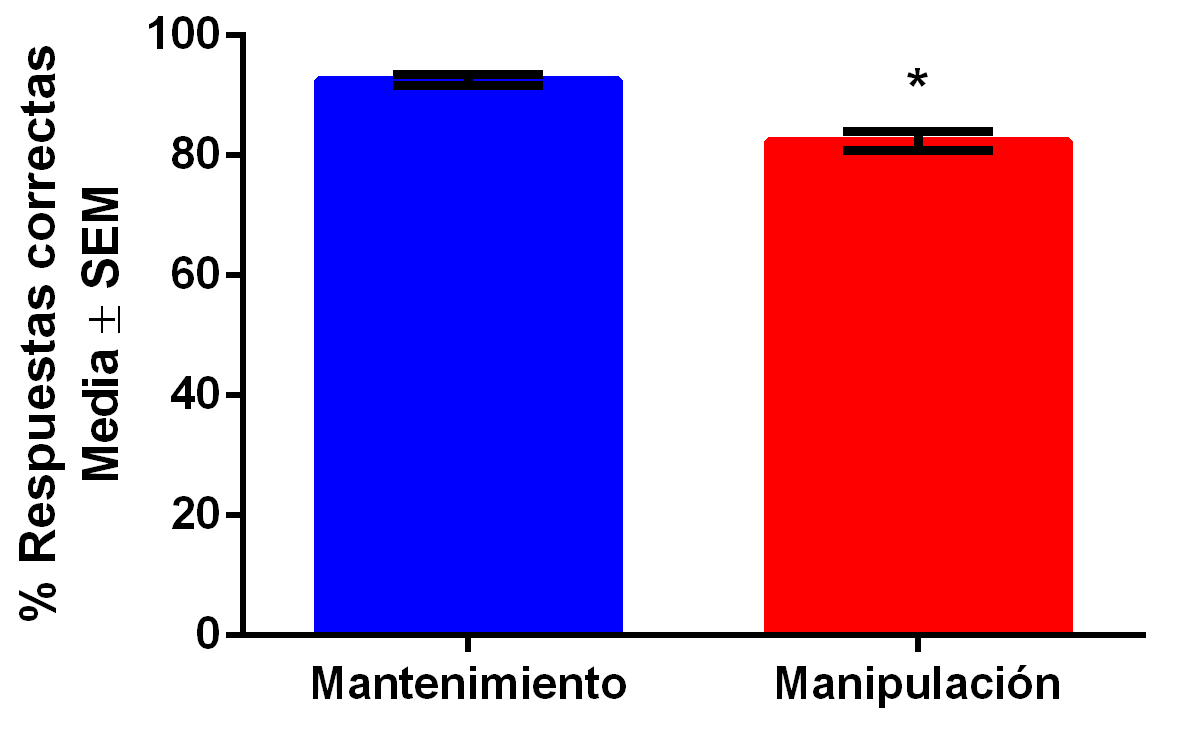
\includegraphics[scale=0.8]{graficas/RC_Tar.png}
	\label{Sub:rctar}
	\end{subfigure}
 \end{footnotesize}
	
	\caption{Porcentaje de Respuestas Correctas. Se presenta en el panel \ref{Sub:rcint} la interacción entre los factores, en el panel \ref{Sub:rctur} las diferencias por turno, y en el panel \ref{Sub:rctar} las diferencias entre los subprocesos de la memoria de trabajo.}
	\label{fig:rc}
\end{figure}

\subsubsection{Indice de discriminación d’ de las tareas}
Se calculó el índice de discriminación d’ entre los estímulos target y non-target de las tareas de memoria de trabajo.  No se observaron diferencias significativas por Turno ($p= 0.55$; Fig. \ref{Sub:dprimtur}), ni interacción significativa ($p= 0.87$; Fig. \ref{Sub:dprimint}). Sólo se encontraron diferencias en función del subproceso, siendo mas eficientes para la tarea de mantenimiento que para la de manipulación (Fig. \ref{Sub:dprimtar}),  $ F (1,56)= 56.88, \eta_{p}^{2}= 0.5,  *p<0.001.$

\begin{figure}[h]
 \begin{footnotesize}
  \begin{subfigure}[a]{.4\textwidth}	
	\centering
	\caption{Interacción de Factores}
	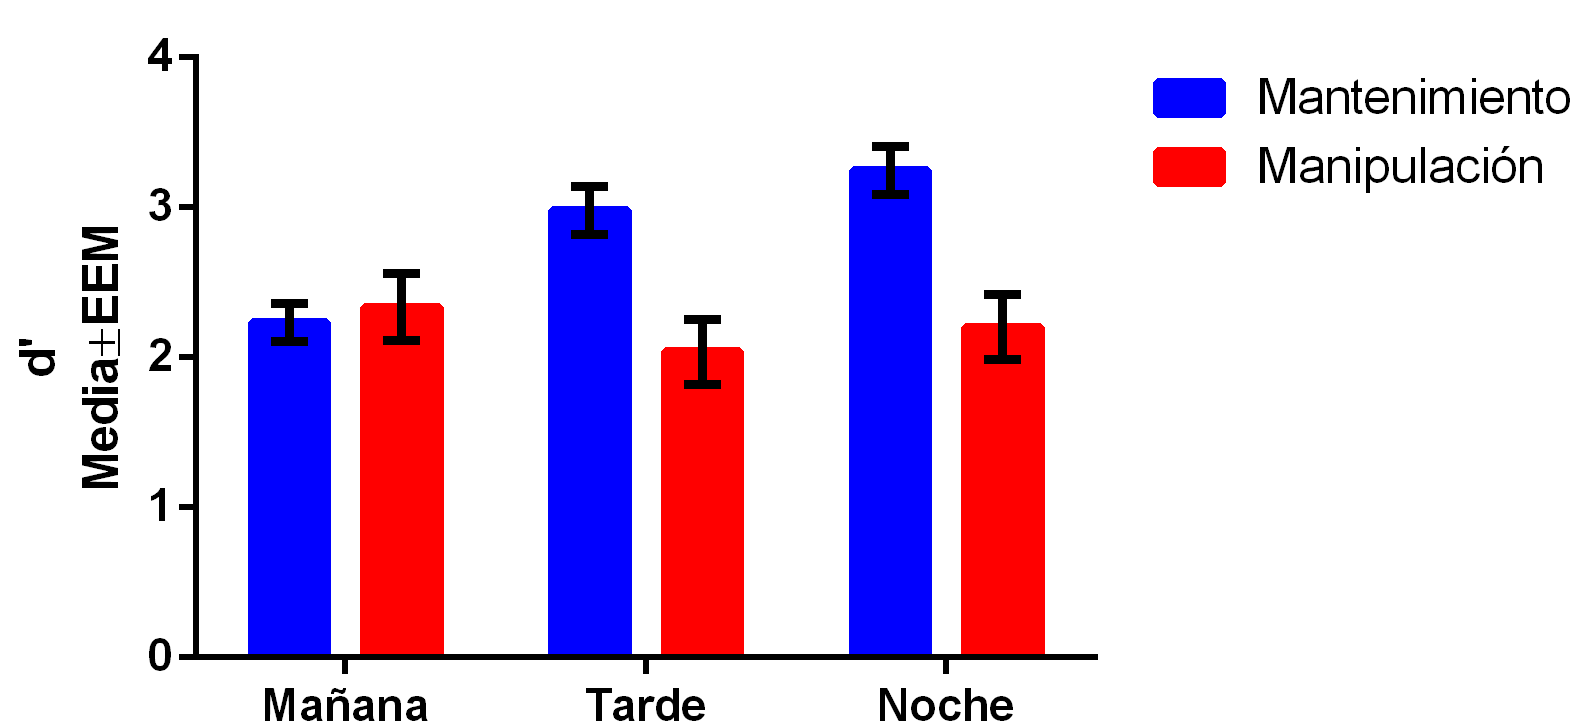
\includegraphics[scale=0.6]{graficas/dprim_intr.png}
	\label{Sub:dprimint}
	\end{subfigure}
    \hfill
    \begin{subfigure}[a]{\textwidth}	
	\centering
	\caption{Entre turnos}
	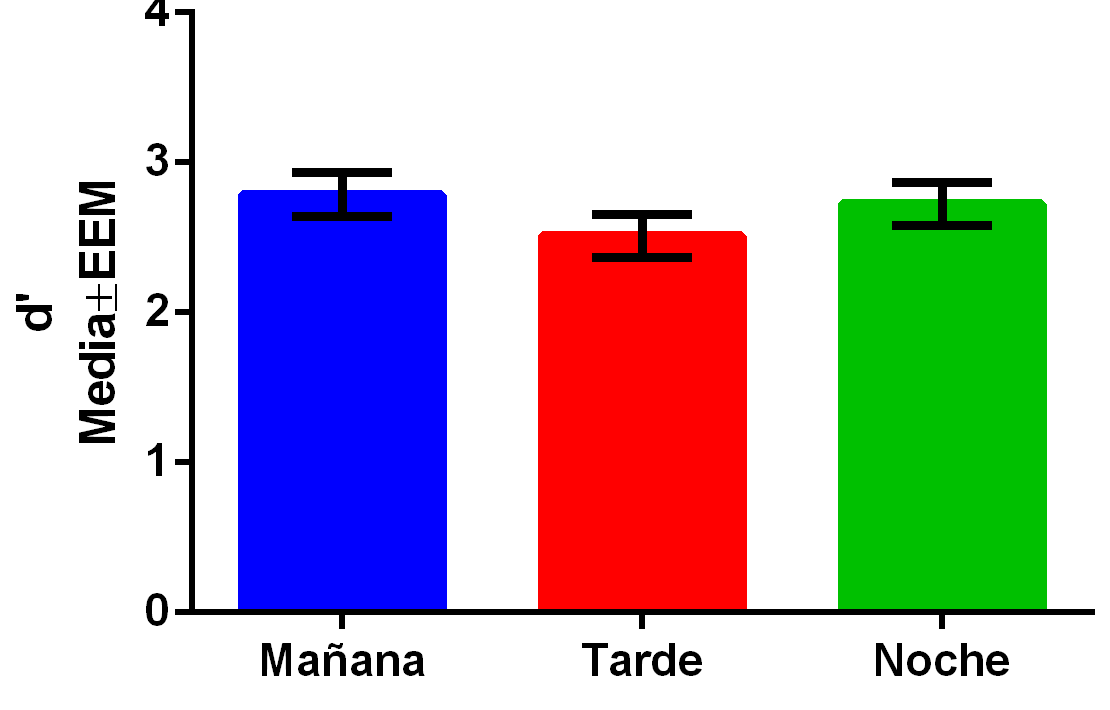
\includegraphics[scale=0.6]{graficas/dprim_Tur.png}
	\label{Sub:dprimtur}
	\end{subfigure}
	
	\begin{subfigure}[b]{0.9\textwidth}	
	\centering
	\caption{En función del subproceso (Mantenimiento vs. Manipulación).}
	\includegraphics[scale=0.8]{graficas/dprim_Tar.png}
	\label{Sub:dprimtar}
	\end{subfigure}
 \end{footnotesize}
	
	\caption{Media\rpm EEM del índice de Discriminación d’ en función del subproceso (Mantenimiento vs. Manipulación de memoria de trabajo) $F(1,56)= 56.88, *p <0.001.$}
	\label{fig:dprim}
\end{figure}

\paragraph{Porcentaje de Cambio}
Como parecía existir una diferencia visual entre turnos de la tarde y noche contra los de la mañana se realizó un análisis del porcentaje de cambio para ver si existía realmente una diferencia. No se encontraron diferencias entre turnos ($p=.93303$; Fig.\ref{fig:PCambio}).

\begin{figure}[h]

	\centering
	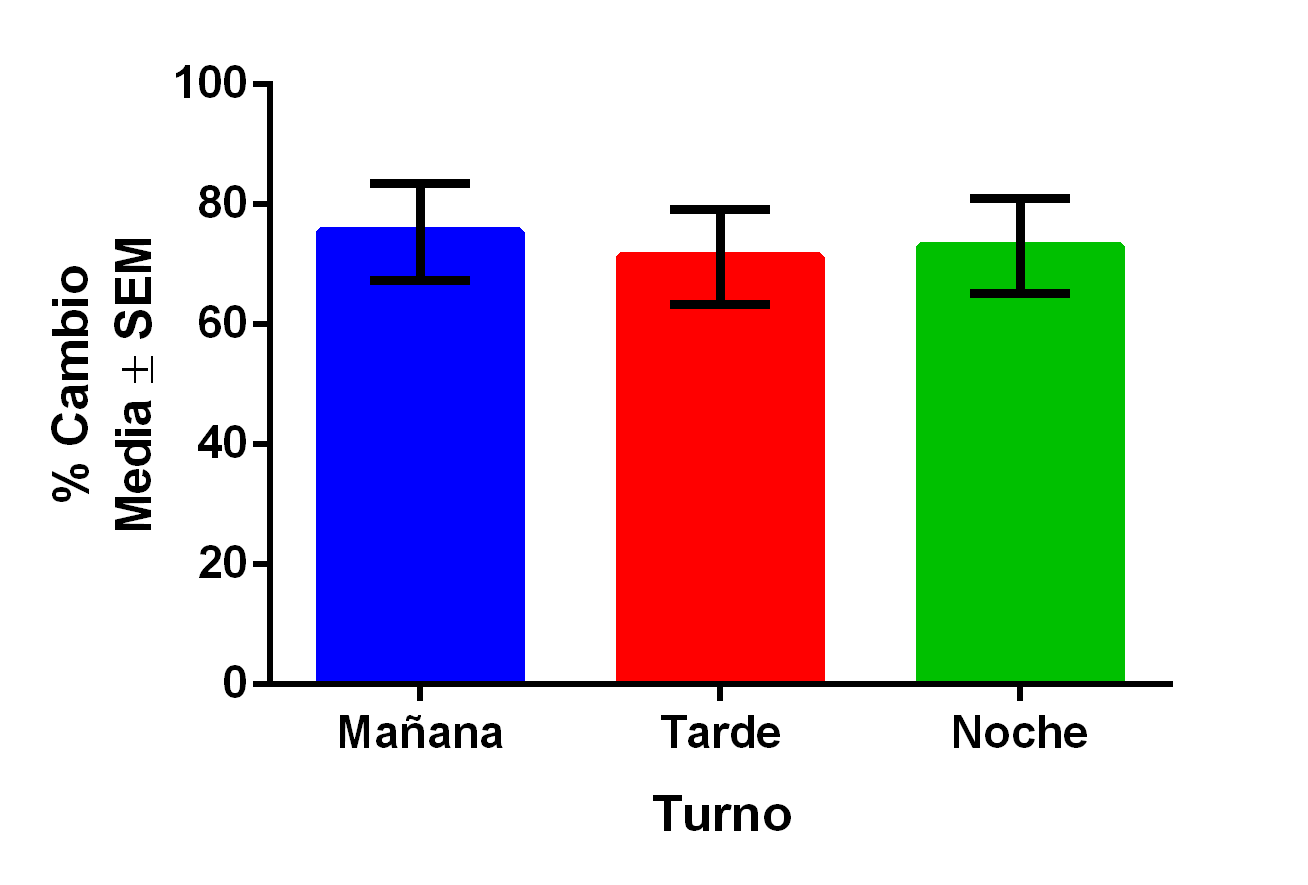
\includegraphics[scale=0.7]{graficas/PCambio.png}
	\caption{Porcentaje de cambio de mantenimiento y manipulación, entre turnos. }
	 	 
	\label{fig:PCambio}
\end{figure}


\subsubsection{Tiempo de Reacción}
Se observaron diferencias significativas en el subproceso, observamos que los sujetos son mas rapidos para responder para la tarea de mantenimiento que para la de manipulación (Mantenimiento vs. Manipulación; Fig. \ref{Sub:rttar})($F (1,56)= 13.53, \eta_{p}^{2}= 0.19, p\textless 0.01$). Pero no se observaron diferencias significativas por Turno ($p=0.09$; Fig. \ref{Sub:rctur}), ni interacción significativa Turno X Subproceso ($p=0.98$; Fig. \ref{Sub:rtint}).

\begin{figure}[h]
 \begin{footnotesize}
  \begin{subfigure}[a]{.4\textwidth}	
	\centering
	\caption{Interacción de Factores}
	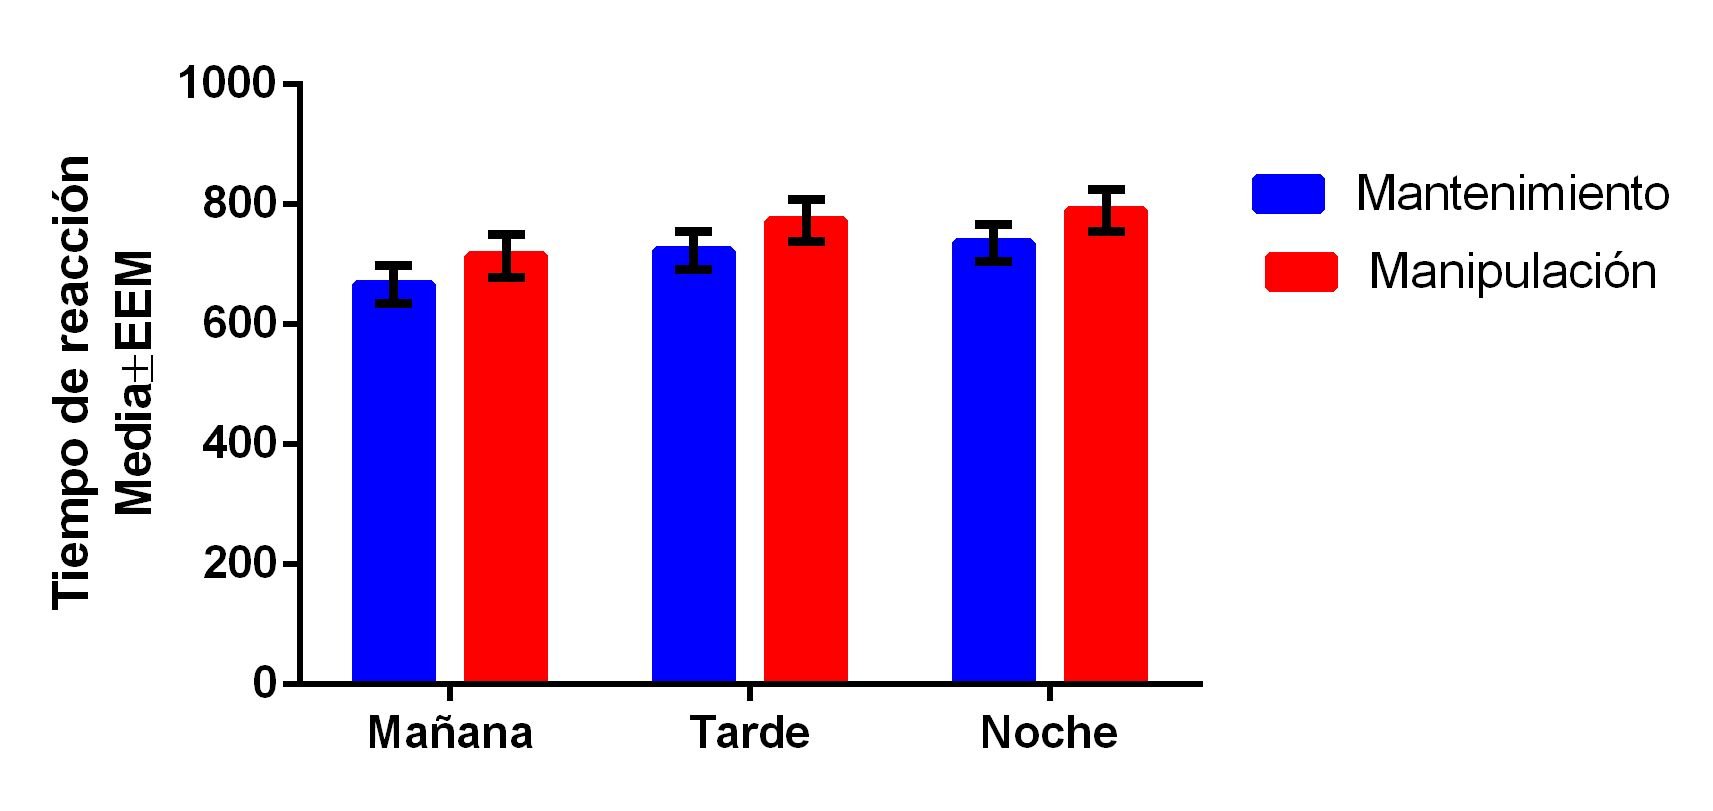
\includegraphics[scale=0.6]{graficas/RT_intr.png}
	\label{Sub:rtint}
	\end{subfigure}
    \hfill
    \begin{subfigure}[a]{\textwidth}	
	\centering
	\caption{Entre turnos}
	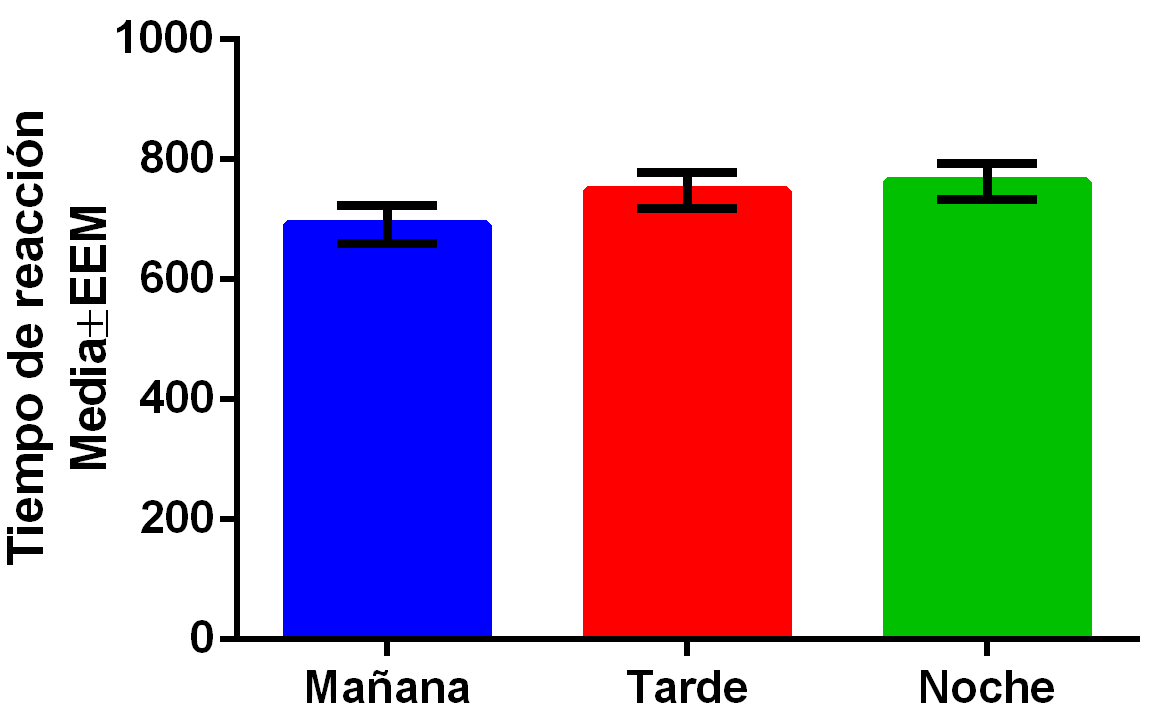
\includegraphics[scale=0.6]{graficas/RT_Tur.png}
	\label{Sub:rttur}
	\end{subfigure}
	
	\begin{subfigure}[b]{0.9\textwidth}	
	\centering
	\caption{En función del subproceso (Mantenimiento vs. Manipulación).}
	\includegraphics[scale=0.8]{graficas/RT_Tar.png}
	\label{Sub:rttar}
	\end{subfigure}
 \end{footnotesize}
	\caption{Tiempo de reacción en función del subproceso de la memoria de trabajo (Mantenimiento vs. Manipulación) $F=(1,56)= 13.53, *p\textless0.01.$}
	\label{fig:rt}
\end{figure}


 
\subsubsection{Tiempo de procesamiento}
Para conocer el tiempo de procesamiento adicional requerido para realizar el mantenimiento y la manipulación de información se contrastó el tiempo de reacción de la tarea control a la tarea de mantenimiento (Fig. \ref{Sub:MtPv}); y el tiempo de reacción de la tarea de mantenimiento a la tarea de manipulación (Fig. \ref{Sub:MpMt}). No encontrando diferencias por turnos ($p=0.85$ y $p=0.99$, respectivamente)

\begin{figure}[h]
 \begin{footnotesize}
  \begin{subfigure}[a]{.4\textwidth}	
	\centering
	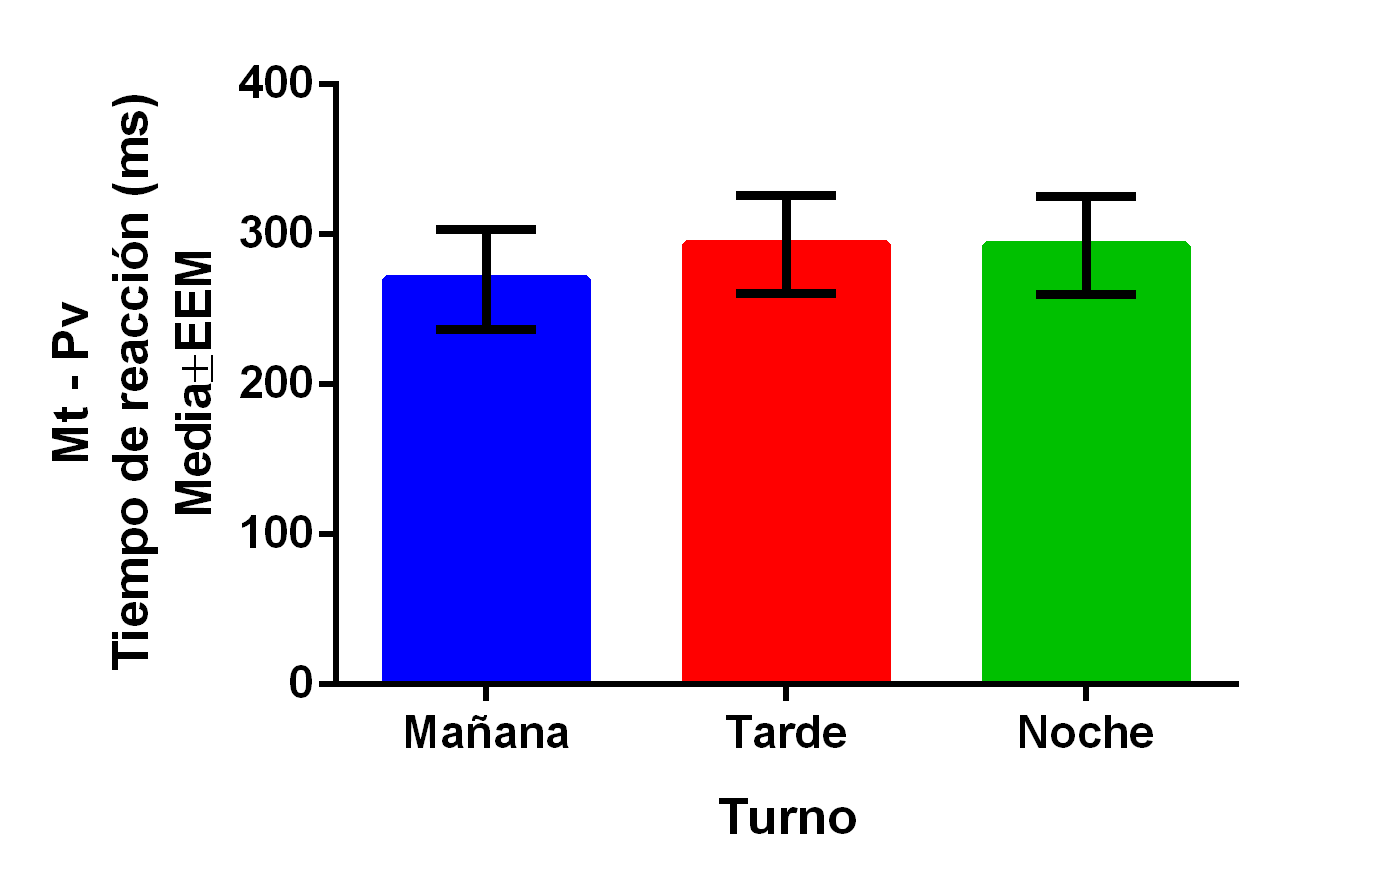
\includegraphics[scale=0.6]{graficas/MtPv.png}
	\caption{Mantenimiento vs. Tarea Control}
	\label{Sub:MtPv}
	\end{subfigure}
    \hfill
    \begin{subfigure}[a]{\textwidth}	
	\centering
	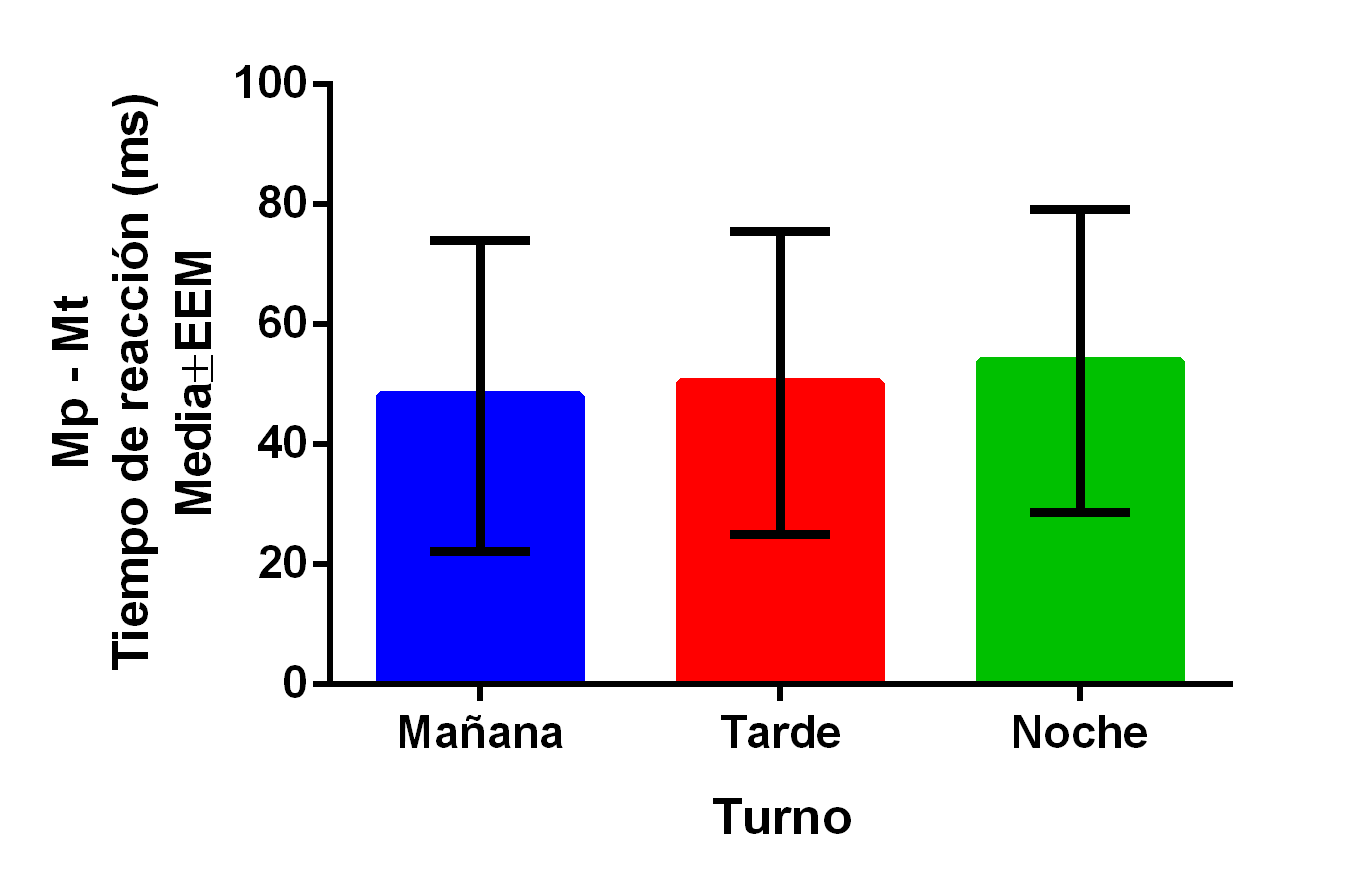
\includegraphics[scale=0.6]{graficas/MpMt.png}
	\caption{Manipulación vs Mantenimiento}
	\label{Sub:MpMt}
	\end{subfigure}
	
 \end{footnotesize}
	\caption{Tiempo de reacción contrastando entre la tarea control y mantenimiento; y el contraste entre Mantenimiento vs. Manipulación }
	\label{fig:pv}
\end{figure}
\clearpage
\newpage 

\section{Discusión}
La presente tesis buscó probar si la eficiencia de la MT para mantener y manipular cambiaba en función de la hora del día. Se encontró que, aunque se observa una disminución en la eficiencia para manipular con respecto a mantener (replicando hallazgos de estudios previos \cite{DEsposito2015, Veltman2003}) evaluado a través porcentaje de respuestas correctas, el tiempo de reacción, el índice d’ y la eficiencia inversa , esto es independiente al momento del día. Además, no se encontraron diferencias a lo largo de los horarios evaluados del día en función del cronotipo ni de la eficiencia general de la MT. Cabe señalar que, aunque nuestra muestra es mayor a otros estudios reportados, las características de la muestra de otros estudios reportados son personas de mayor edad, con rutinas fijas, por lo que los efectos del momento del día sobre la eficiencia en memoria de trabajo pueden ya estar establecidos de manera clara.


En esta investigación se controló la cantidad de personas de un tipo de cronotipo en cada grupo para eliminar la posible interferencia o efecto de éste sobre la cognición que se ha reportado \cite{Schmidt2015} y efectivamente encontrar diferencias en función de variaciones diurnas, de haberlas. La muestra que se evaluó en su mayoría tuvo cronotipo indiferenciado y esto podría deberse a que la mayoría de los participantes cursan la licenciatura, demanda que implica la función idónea en horarios mixtos y quizá por ello no se observan diferencias. Previamente se ha reportado que los estudiantes universitarios tienen horarios de comida y de sueño irregulares \cite{Lund2010} lo cual tiene repercusiones en la capacidad de sincronización circadiana dificultando el ajustarse al periodo de 24 horas de manera adecuada \cite{Harma1993}. Otro factor que podría influir en la ciclicidad cognoscitiva es la iluminación a la que son expuestos los individuos ya que se ha reportado, que el uso de pantallas o la iluminación ambiental genera una modificación en la fase circadiana de las personas \cite{Chang2015,Chang2011,Gronfier2007}. Aunque los hábitos de sueño en esta población son malos y se encuentran expuestos por más tiempo a luz artificial, por el hecho de realizar las tareas escolares hasta tarde, sin embargo eso no parece representar una limitante en la vida diaria de nuestros participantes pues todos se encuentran en altos niveles de eficiencia, parece ser que únicamente la disminución en horas de sueño es un efecto del intento los participantes por llegar a las 7 am, más que un fenómeno recurrente en sus vidas, esto se puede corroborar al contrastar las horas dormidas habitualmente de los participantes, donde todos tienen una media de 6 horas al día (ver tabla \ref{tab:CaracSoci}).
 


Adicionalmente, el método de momento del día difiere de otros métodos de estudio, como el de rutina constante o desincronización forzada, donde se mantiene al participante en el laboratorio bajo condiciones de alimentación, sueño y actividad controladas. Además de que se suele privar a los sujetos de sueño, lo cual podría estar forzando las diferencias observadas en esos estudios, ya que se ha mostrado que el tiempo que llevan privadas de sueño las personas es un factor que implica un decremento en la eficiencia \cite{Wright2002}. También es posible que la tarea empleada en esta tesis resultara muy sencilla para los participantes, ya que los porcentajes de respuestas correctas están por encima del 80\%. Esta tesis difiere de estudios previos \cite{Baddeley1970,Schmidt2015}, al evaluar en tres momentos del día, separar en subprocesos de mantener y manipular información, y evaluar la eficiencia de forma independiente al cronotipo de los participantes. Cabe destacar que nuestros participantes mostraron inteligencia promedio para su edad acorde a la Escala Breve de Inteligencia Shipley-2 \cite{Shipley2014} y no difieren en variables demográficas. Lo cual nos señala que, aunque literatura reporta que existe una diferencia a lo largo del día; en población mexicana en edad universitaria estas diferencias no se presentan al separarse del efecto del cronotipo. Lo que nos permite llevar a cabo estudios de desempeño cognitivo en diferentes momentos del día sin que esto represente una variable que modifique el resultado a obtener.


\section{Limitaciones y sugerencias}
Una de las principales limitantes de nuestra investigación es que los sujetos son evaluados una sola vez en el día, ya que pueden existir diferencias individuales en el desempeño a lo largo del día, y disminuir así la varianza ambiental que pueda existir. Por lo que se sugiere realizar una evaluación repetida de los mismos sujetos en varios momentos del día. También se sugiere evaluar los niveles de cortisol en sangre como una medida para evaluar el estado de reloj circadiano de los participantes, así como evaluar las horas de sueño y de ingesta de alimento de los participantes, cuando menos una semana antes, para tener una descripción más precisa de estás. El hacer hincapié en mantener las horas de sueño estables el día de la sesión con las horas habituales también se sugiere como medida para evitar algún factor adicional, que si bien no se observo influencia de esta diferencia en los resultados obtenidos en la presente tesis, nos daría una mayor certeza en cuanto a los resultados.   También es importante intentar reducir la exposición a pantallas e iluminación ambiental que re-sincronice el reloj interno, o utilizar las herramientas disponibles que disminuyen este efecto.  Para lograr tales puntos se recomienda el uso de un dispositivo de tipo Actiwatch, que permiten cuantificar las horas de actividad, sueño, y exposición a la luz en las personas \cite{Figueiro2013}.

Incrementar la dificultad de las tareas al añadir, por ejemplo, más características a los estímulos, podría ayudar a acentuar las posibles diferencias entre horarios a lo largo del día.
 
\section{Conclusiones}


Los resultados de esta tesis sugieren que no existe una asociación entre las variaciones diurnas y la eficiencia en el mantenimiento y la manipulación de información en la memoria de trabajo independientemente del cronotipo. Sin embargo, se observan resultados que coinciden con la literatura previa en memoria de trabajo encontrando mayor dificultad en manipular que en mantener. Si bien, no se encuentra efecto del momento del día sobre la eficiencia de la memoria de trabajo. Es posible que estas diferencias reportadas previamente puedan deberse a otro tipo de procesos cognoscitivos  o biológicos y no necesariamente el mantenimiento y/o la manipulación de información de la memoria de trabajo.

   




\renewcommand{\baselinestretch}{1}
\bibliography{mendeley_v2}

\bibliographystyle{apacite}



\end{document}
